\documentclass{beamer} 
\usepackage{amsmath,amsthm}
\usepackage{graphicx,microtype,parskip}
\usepackage{caption,subcaption,multirow}
\usepackage{attrib}

\frenchspacing

\usetheme{default}
\usecolortheme{whale}

\setbeamertemplate{navigation symbols}{}

\setbeamercolor{title}{fg=blue,bg=white}

\setbeamercolor{block title}{fg=white,bg=gray}
\setbeamercolor{block body}{fg=black,bg=lightgray}

\setbeamercolor{block title alerted}{fg=white,bg=darkgray}
\setbeamercolor{block body alerted}{fg=black,bg=lightgray}


\title{The changing functional composition of the North American species pool}
\subtitle{modeling species origination-extinction as a function of functional group and environmental context}
\author{Peter D Smits}
\institute{Committee on Evolutionary Biology, University of Chicago}
\titlegraphic{
  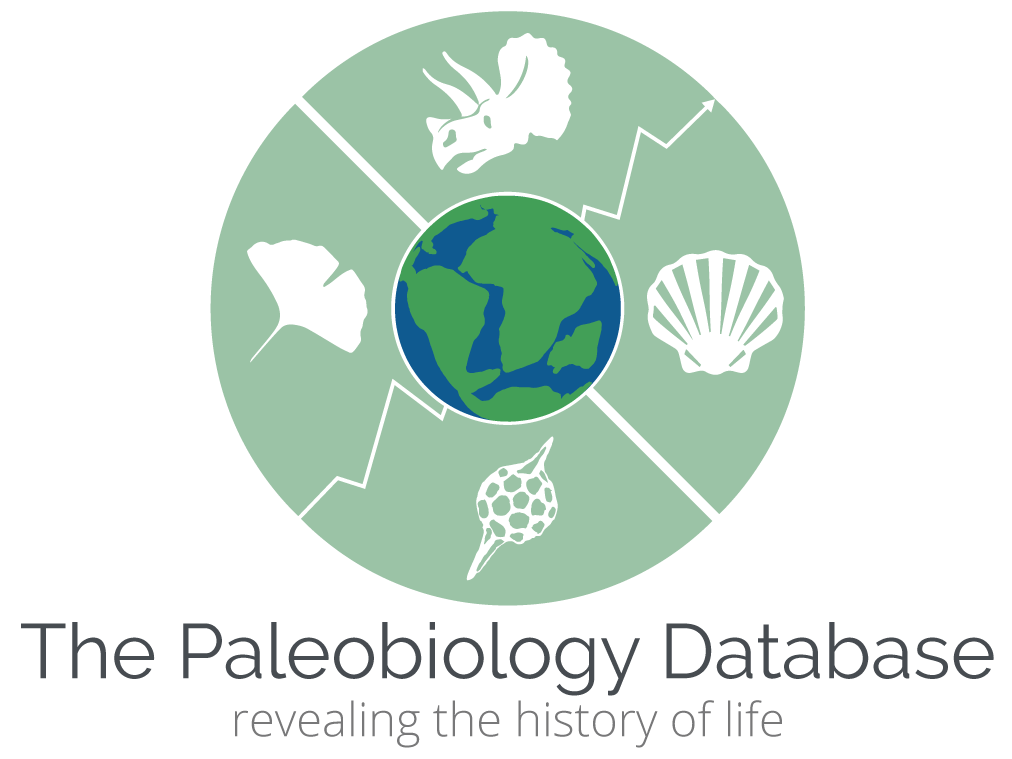
\includegraphics[width=2.75cm,height=2.75cm,keepaspectratio=true]{figure/paleodb}
  \hspace*{0.35\paperwidth}
  
\includegraphics[width=2cm,height=2cm,keepaspectratio=true]{figure/chicago}
}
\date{}

\begin{document}

\begin{frame}
  \maketitle
\end{frame}


\begin{frame}
  \begin{alertblock}{Question}
    When are certain ecologies, ecotypes, or functional groups enriched or depleted in a species pool?
  \end{alertblock}
\end{frame}

\begin{frame}
  \frametitle{Species pool concept}

  \begin{center}
    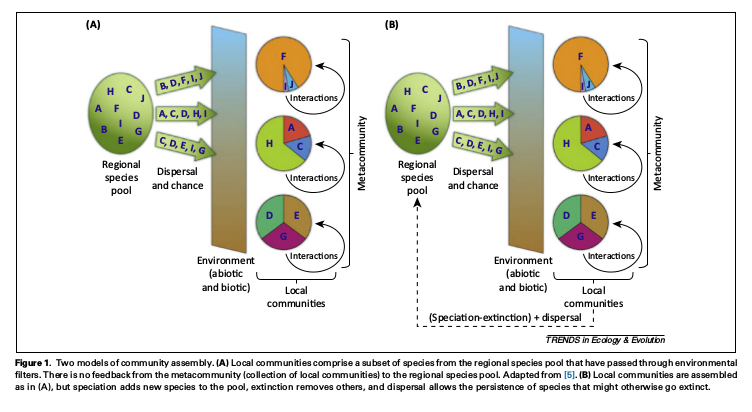
\includegraphics[height=0.8\textheight,width=\textwidth,keepaspectratio=true]{figure/schemske_pool}
  \end{center}

  \attrib{\footnotesize{Mittelbach and Schemske, 2015, \em{TREE}}}
\end{frame}

\begin{frame}
  \frametitle{Functional groups}

  \begin{center}
    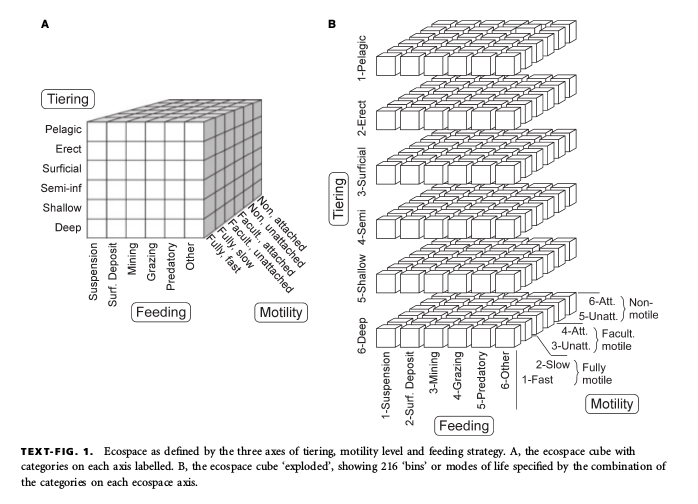
\includegraphics[height=0.8\textheight,width=\textwidth,keepaspectratio=true]{figure/ecocube}
  \end{center}

  \tiny{\attrib{Bambach \em{et al.} 2007 \em{Palaeontology}}}
\end{frame}

\begin{frame}
  \frametitle{Structured data in biology; the fourth-corner problem}

  \begin{center}
    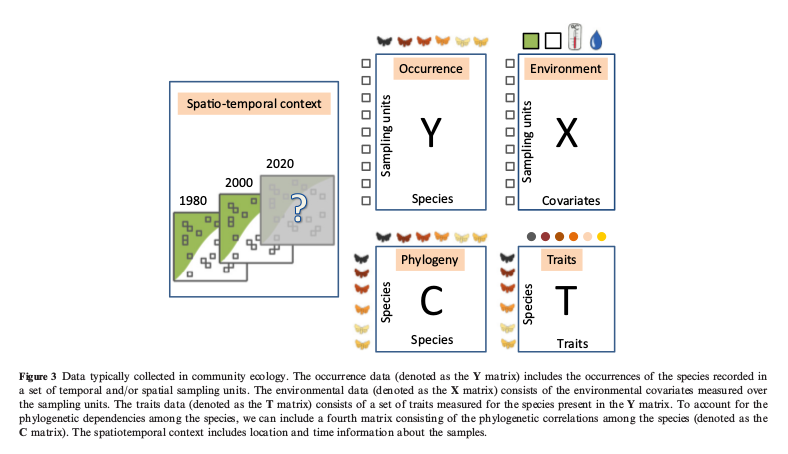
\includegraphics[width = \textwidth,height = 0.8\textheight,keepaspectratio = true]{figure/ovaskainen_data}
  \end{center}

  \tiny{\attrib{Ovaskainen \textit{et al.} 2017 \em{Ecology Letters}}}
\end{frame}


\begin{frame}
  \frametitle{Age of Mammals}
  \begin{center}
    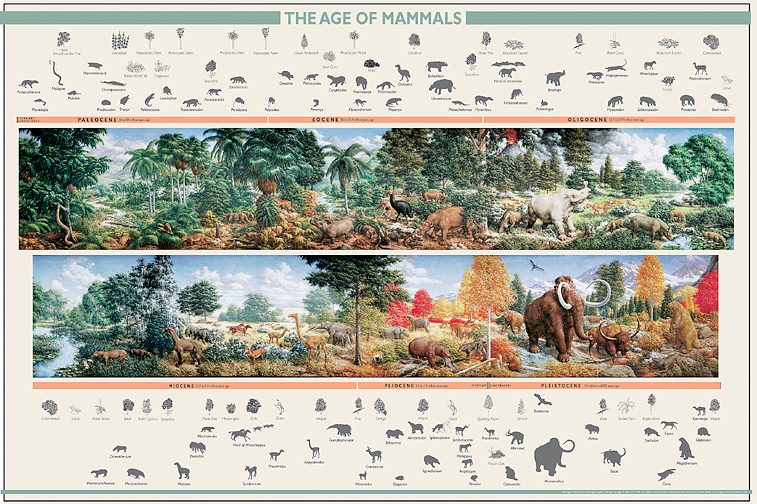
\includegraphics[width = \textwidth,height = 0.8\textheight,keepaspectratio = true]{figure/aom}
  \end{center}
\end{frame}


\begin{frame}
  \frametitle{Differences in extinction risk}

  \begin{center}
    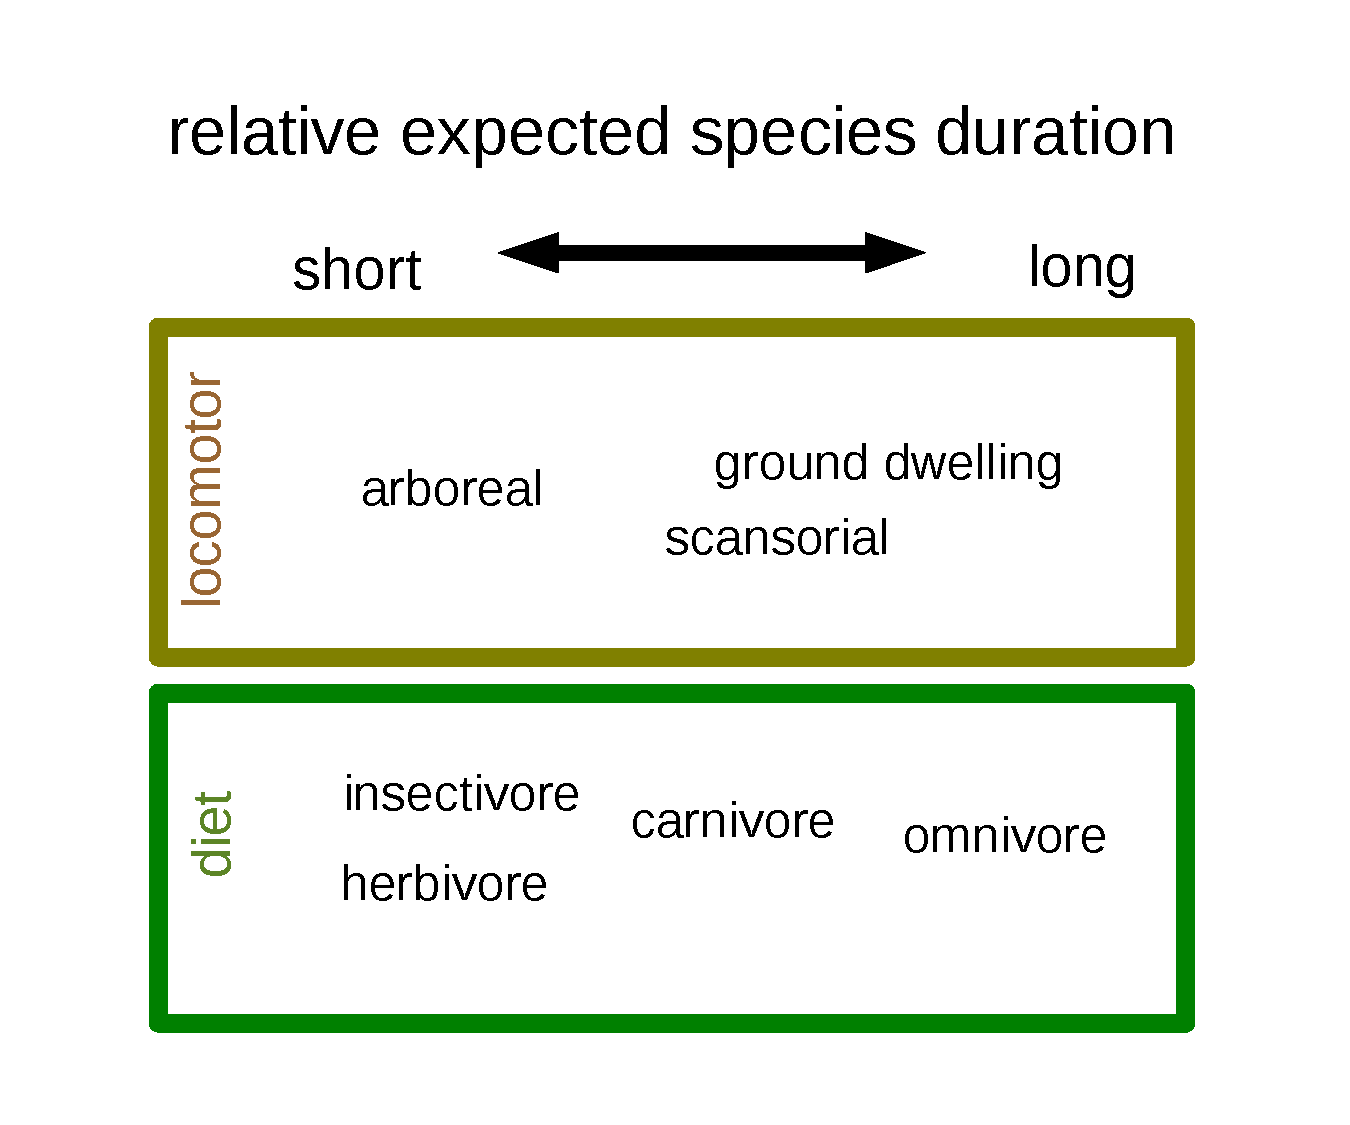
\includegraphics[height=0.8\textheight,width=\textwidth,keepaspectratio=true]{figure/smits_2015_results}
  \end{center}

  \attrib{\footnotesize{Smits 2015 \em{PNAS}}}
\end{frame}

%\begin{frame}
%  \frametitle{Functional groups over time}
%
%  \begin{center}
%    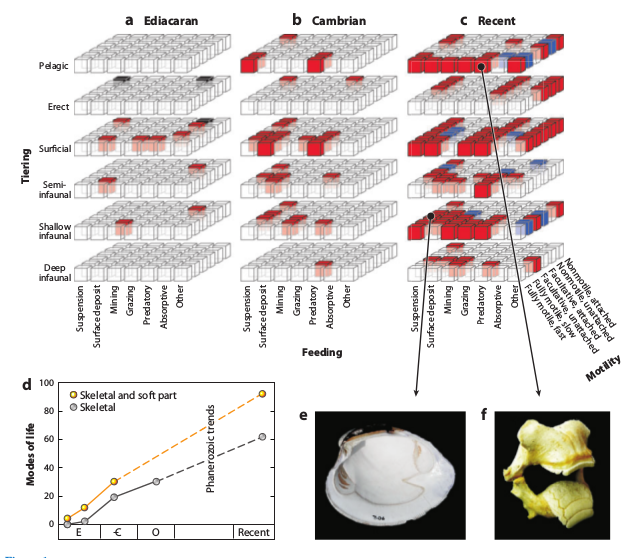
\includegraphics[height=0.8\textheight,width=\textwidth,keepaspectratio=true]{figure/bush_cube_time}
%  \end{center}
%
%  \tiny{\attrib{Bush and Bambach 2011 \em{Annu. Rev. Earth Planet Sci.}}}
%\end{frame}

%\begin{frame}
%  \frametitle{Models of structured data}
%
%  \begin{center}
%    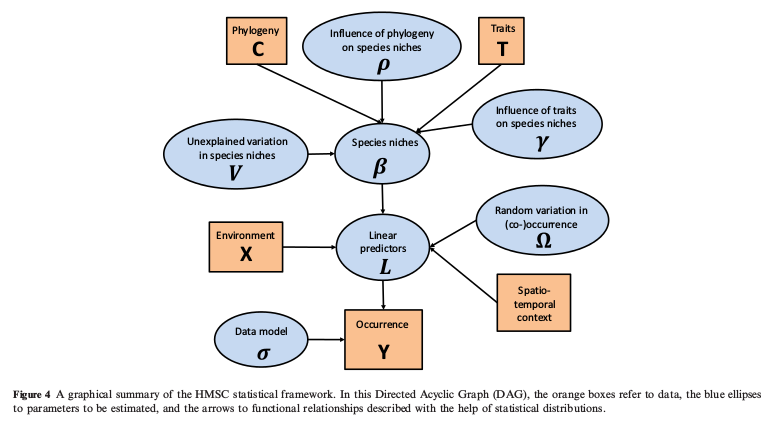
\includegraphics[width = \textwidth,height = 0.8\textheight,keepaspectratio = true]{figure/ovaskainen_dag}
%  \end{center}
%
%  \tiny{\attrib{Ovaskainen \textit{et al.} 2017 \em{Ecology Letters}}}
%\end{frame}

%\begin{frame}
%  \frametitle{The fourth-corner problem}
%
%  \begin{center}
%    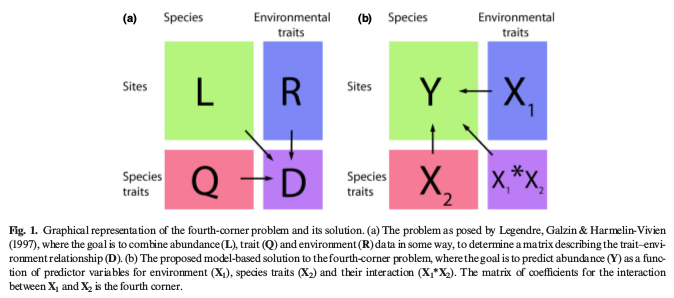
\includegraphics[height=0.8\textheight,width=\textwidth,keepaspectratio=true]{figure/warton_fourth_corner}
%  \end{center}
%
%  \attrib{\footnotesize{Brown \em{et al.}, 2014, \em{Methods Ecol. Evol.}}}
%\end{frame}


\begin{frame}
  \frametitle{Covariates of interest}
  \begin{columns}
    \begin{column}{0.5\textwidth}
      individual-level \\(species i at time unit t)
      \begin{itemize}
        \item effect of locomotor type
          \begin{itemize}
            \item arboreal, digitigrade, plantigrade, unguligrade, fossorial, scansorial
          \end{itemize}
        \item effect of dietary type
          \begin{itemize}
            \item carnivore, herbivore, insectivore, omnivore
          \end{itemize}
        \item effect body size \\(rescaled log body mass)
      \end{itemize}
    \end{column}
    \begin{column}{0.5\textwidth}
      group-level (2 My time unit t)
      \begin{itemize}
        \item temperature record based on Mg/Ca estimates
          \begin{itemize}
            \item mean and range \\(rescaled log degrees)
          \end{itemize}
        \item plant community phase following Graham 2011
      \end{itemize}
    \end{column}
  \end{columns}
\end{frame}

%\begin{frame}
%  \frametitle{Model of taxon occurrence}
%  \begin{itemize}
%    \item response is p/a of genus in NA at time \(t\)
%      \begin{itemize}
%        \item Bernoulli variable 
%        \item probability is (observation prob) times (``true'' presence)
%      \end{itemize}
%    \item observation probability is effect of sampling/fossil record
%      \begin{itemize}
%        \item basic model does not model sampling
%      \end{itemize}
%    \item the latent discrete ``true'' presence modeled as a \\multi-level logistic regression
%      \begin{itemize}
%        \item individual- and group-level
%      \end{itemize}
%  \end{itemize}
%\end{frame}

\begin{frame}
  \frametitle{Paleo-fourth corner model}

  \begin{center}
    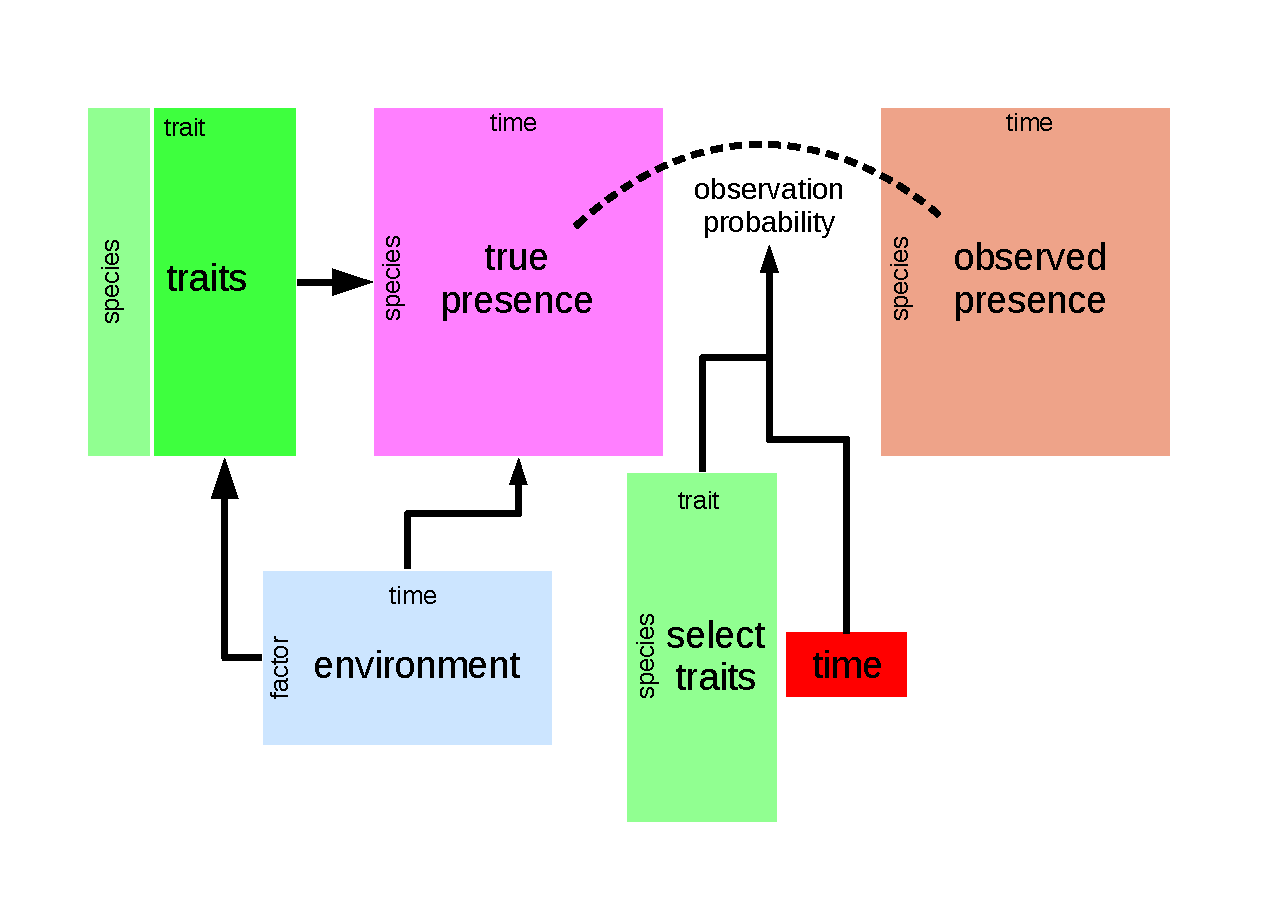
\includegraphics[height=0.8\textheight,width=\textwidth,keepaspectratio=true]{figure/paleo_fourth_corner}
  \end{center}
\end{frame}


\begin{frame}
  \frametitle{Model and sampling statement definition}
  \begin{center}
    \begin{scriptsize}
      \begin{columns}
        \begin{column}{0.5\textwidth}
          \begin{align*}
            y_{i, t} &\sim \text{Bernoulli}(p_{i, t} z_{i, t}) \\
            p_{i, t} &= \text{logit}^{-1}(\alpha_{0} + \alpha_{1} m_{i} + r_{t}) \\ 
            r_{t} &\sim \mathcal{N}(0, \sigma) \\
            \alpha_{0} &\sim \mathcal{N}(0, 1) \\
            \alpha_{1} &\sim \mathcal{N}(1, 1) \\
            \sigma &\sim \mathcal{N}^{+}(1) \\
            z_{i, 1} &\sim \text{Bernoulli}(\phi_{i, 1}) \\
            z_{i, t} &\sim \text{Bernoulli}\left(z_{i, t - 1} \pi_{i,t} + \sum_{x = 1}^{t}(1 - z_{i, x}) \phi_{i,t}\right) \\
            \phi_{i, t} &= \text{logit}^{-1}(a^{\phi}_{t, j[i]} + b^{\phi}_{1} m_{i} + b^{\phi}_{2} m_{i}^{2}) \\
            \pi_{i, t} &= \text{logit}^{-1}(a^{\pi}_{t, j[i]} + b^{\pi}_{1} m_{i} + b^{\pi}_{2} m_{i}^{2}) \\
            a^{\phi} &\sim \text{MVN}(U \gamma^{\phi}, \Sigma^{\phi}) \\
            a^{\pi} &\sim \text{MVN}(U \gamma^{\pi}, \Sigma^{\pi}) \\
          \end{align*}
        \end{column}
        \begin{column}{0.5\textwidth}
          \begin{align*}
            \Sigma^{\phi} &= \text{diag}(\tau^{\phi}) \Omega^{\phi} \text{diag}(\tau^{\phi}) \\
            \Sigma^{\pi} &= \text{diag}(\tau^{\pi}) \Omega^{\pi} \text{diag}(\tau^{\pi}) \\
            \rho &\sim \text{U}(0, 1) \\
            b^{\phi}_{1} &\sim \mathcal{N}(0, 1) \\
            b^{\pi}_{1} &\sim \mathcal{N}(0, 1) \\
            b^{\phi}_{2} &\sim \mathcal{N}(-1, 1) \\
            b^{\pi}_{2} &\sim \mathcal{N}(-1, 1) \\
            \gamma^{\phi} &\sim \mathcal{N}(0, 1) \\
            \gamma^{\pi} &\sim \mathcal{N}(0, 1) \\
            \tau^{\phi} &\sim \mathcal{N}^{+}(1) \\
            \tau^{\pi} &\sim \mathcal{N}^{+}(1) \\
            \Omega^{\phi} &\sim \text{LKJ}(2) \\
            \Omega^{\pi} &\sim \text{LKJ}(2). \\
          \end{align*}
        \end{column}
      \end{columns}
    \end{scriptsize} 
  \end{center}
\end{frame}

%\begin{frame}
%  \frametitle{Paleo-fourth corner model}
%
%  \begin{center}
%    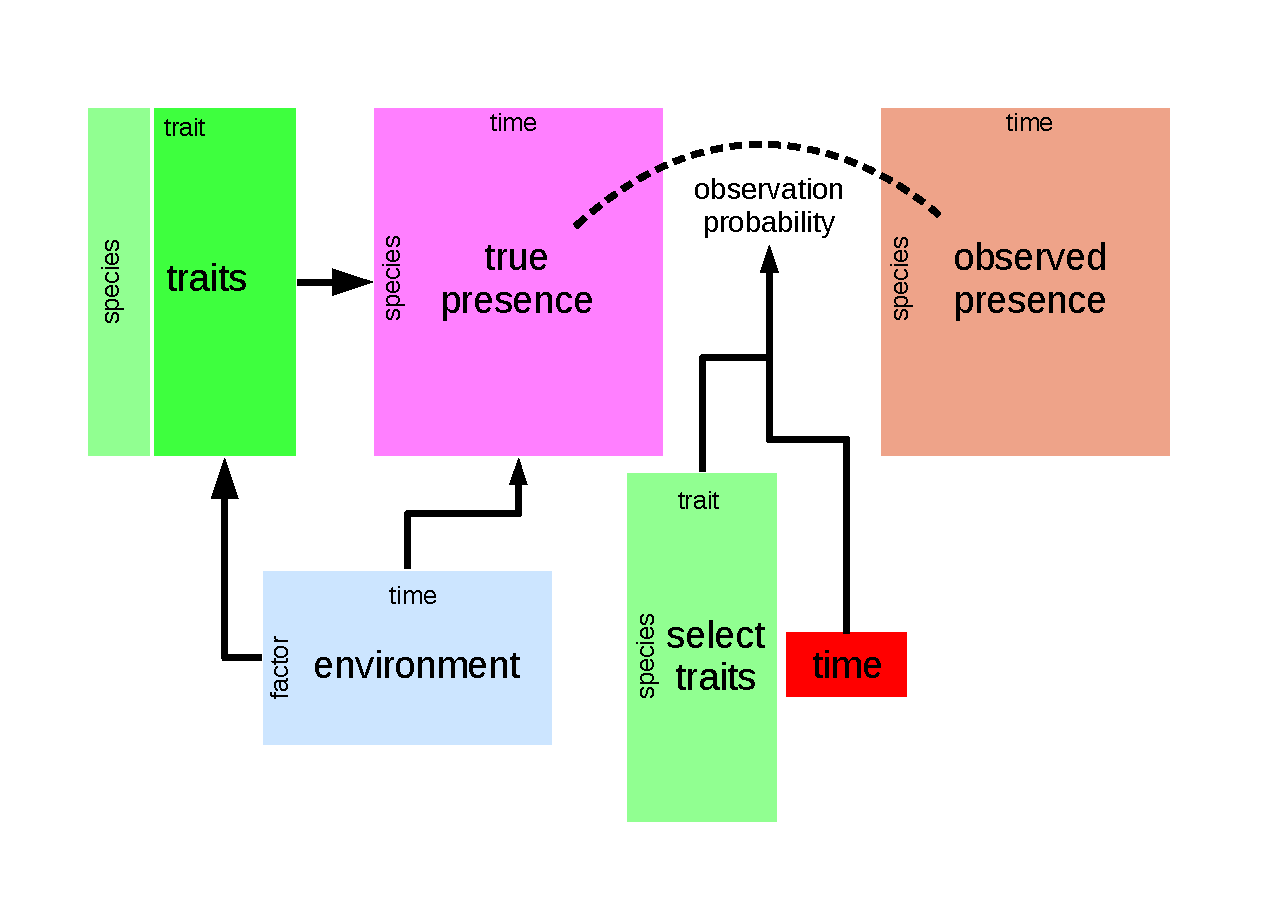
\includegraphics[height=0.8\textheight,width=\textwidth,keepaspectratio=true]{figure/paleo_fourth_corner}
%  \end{center}
%\end{frame}


\begin{frame}
  \frametitle{Bayesian inference and statistics}

  \begin{columns}
    \begin{column}{0.45\textwidth}
      \begin{itemize}
        \item flexible, expressive, intuitive
        \item regularize, partial pooling, external information
        \item Stan probabilistic programming language
          \begin{itemize}
            \item \textbf{Hamiltonian Monte Carlo}
            \item Automatic Differentiation Variational Inference
          \end{itemize}
      \end{itemize}
    \end{column}
    \begin{column}{0.55\textwidth}
      
\includegraphics[height=0.9\textheight,width=\textwidth,keepaspectratio=true]{figure/stan_logo}
    \end{column}
  \end{columns}
\end{frame}

\begin{frame}
  \frametitle{Probability of ecotype origination}
  \begin{center}
    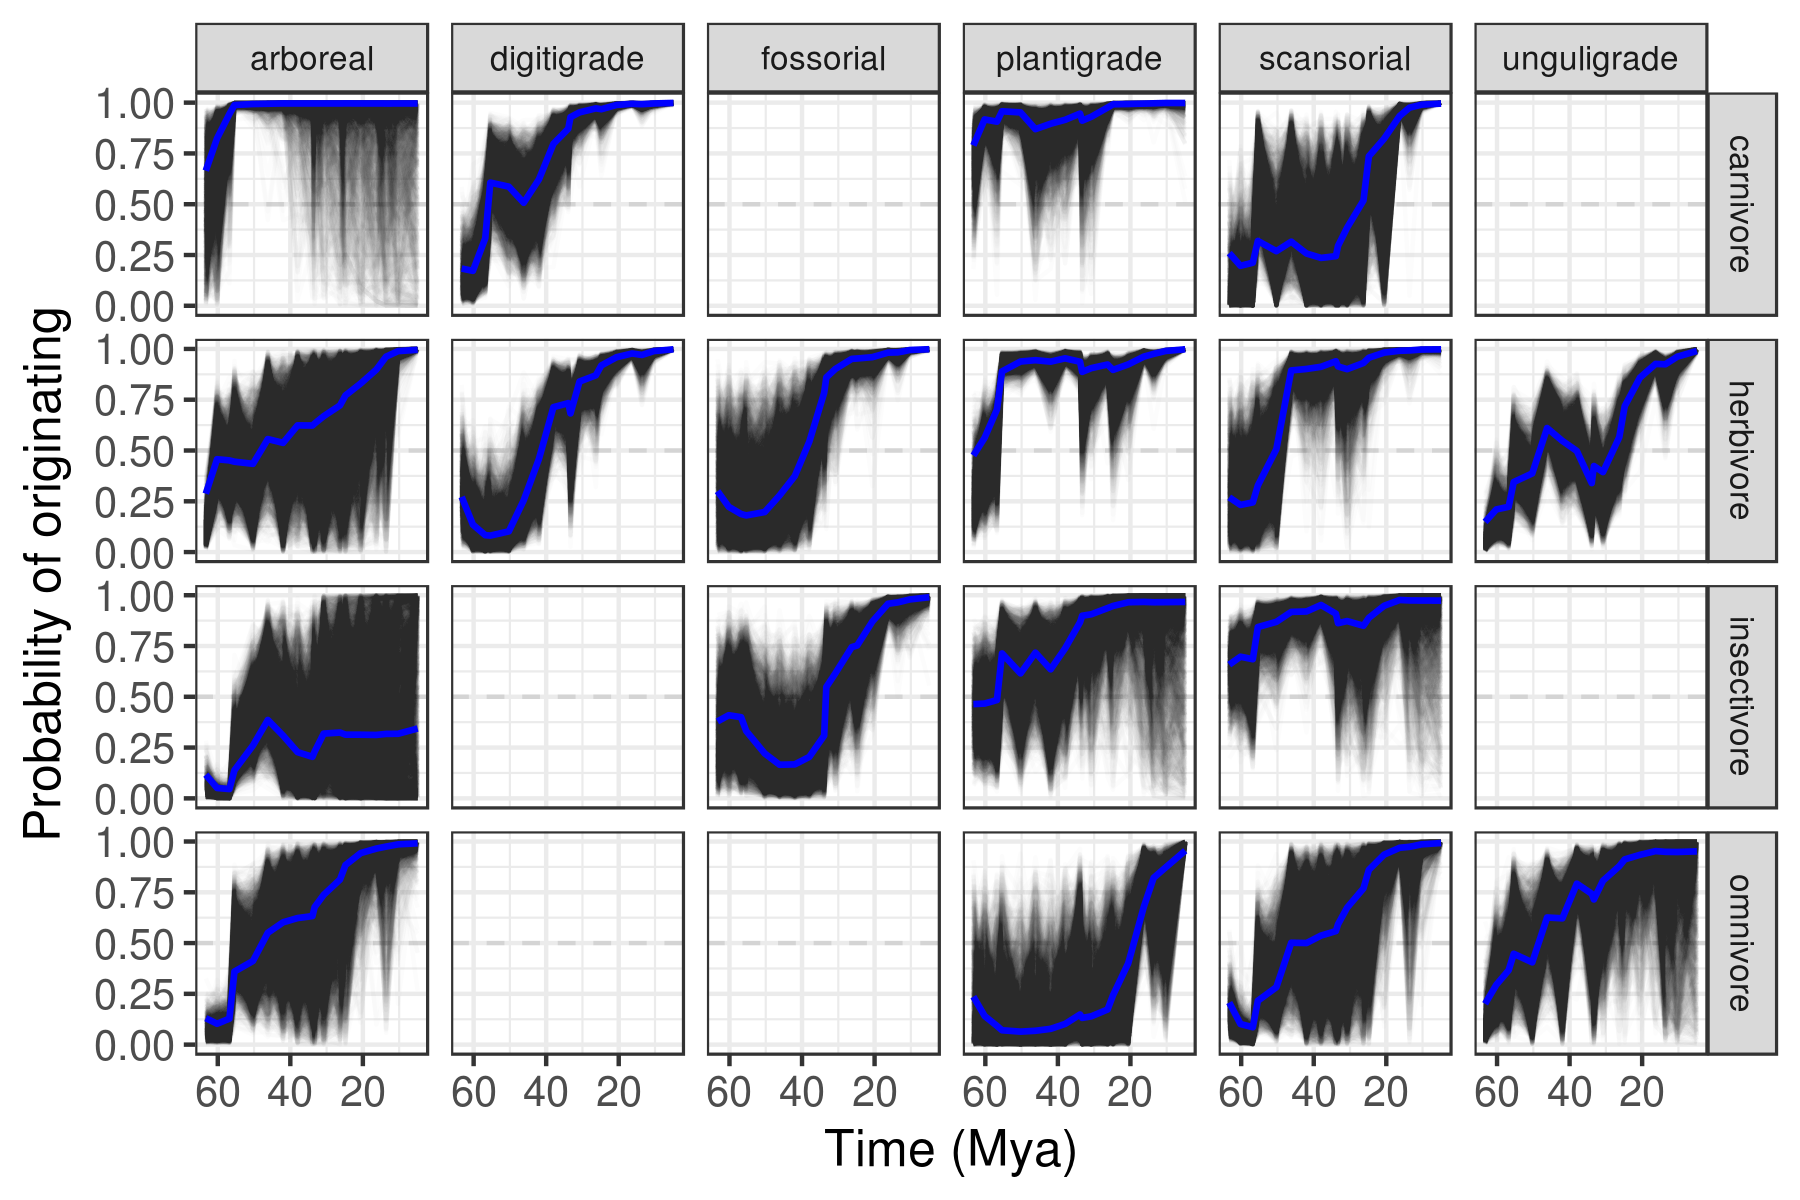
\includegraphics[height=0.8\textheight,width=\textwidth,keepaspectratio=true]{figure/ecotype_origin_bd}
  \end{center}
\end{frame}

\begin{frame}
  \frametitle{Probability of ecotype survival}
  \begin{center}
    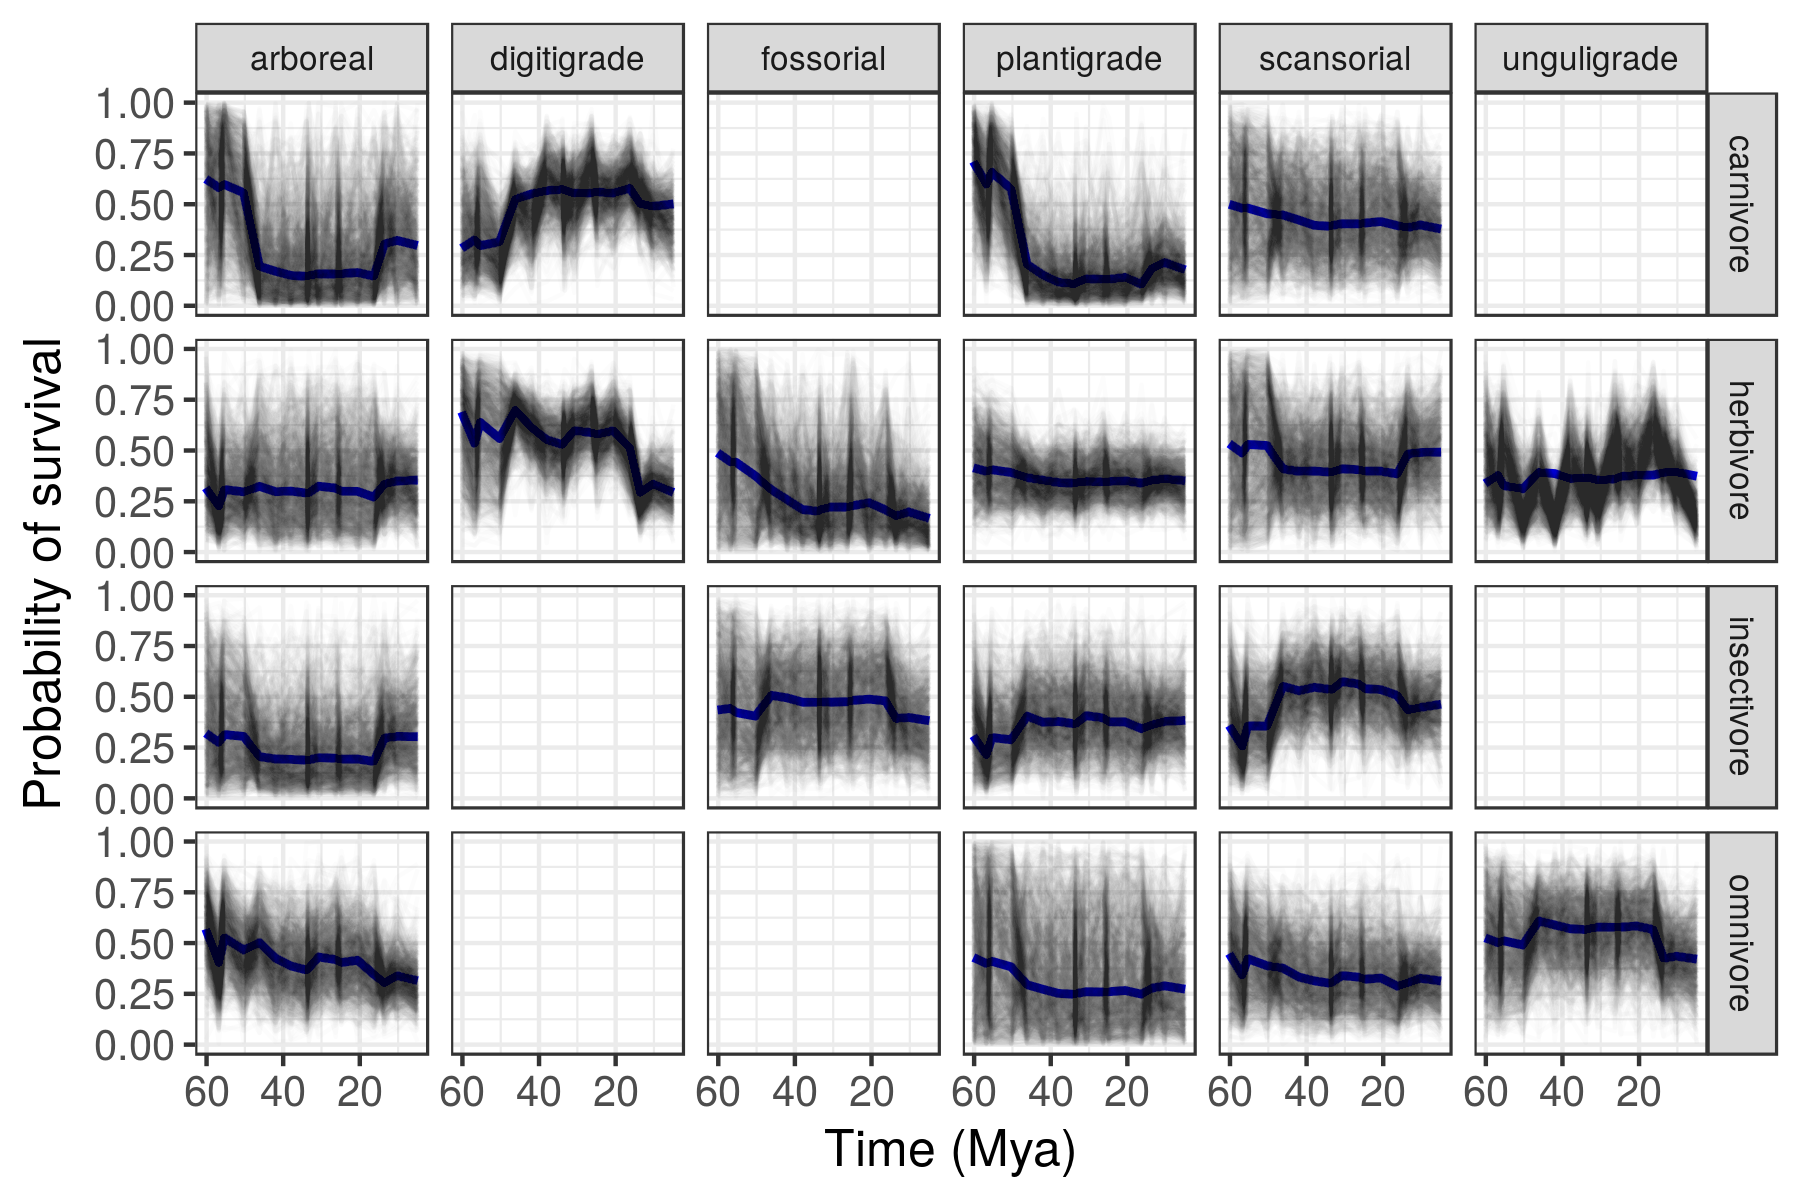
\includegraphics[height=0.8\textheight,width=\textwidth,keepaspectratio=true]{figure/ecotype_survival_bd}
  \end{center}
\end{frame}

\begin{frame}
  \frametitle{Group-level effects (plant phase, climate) on origination}
  \begin{center}
    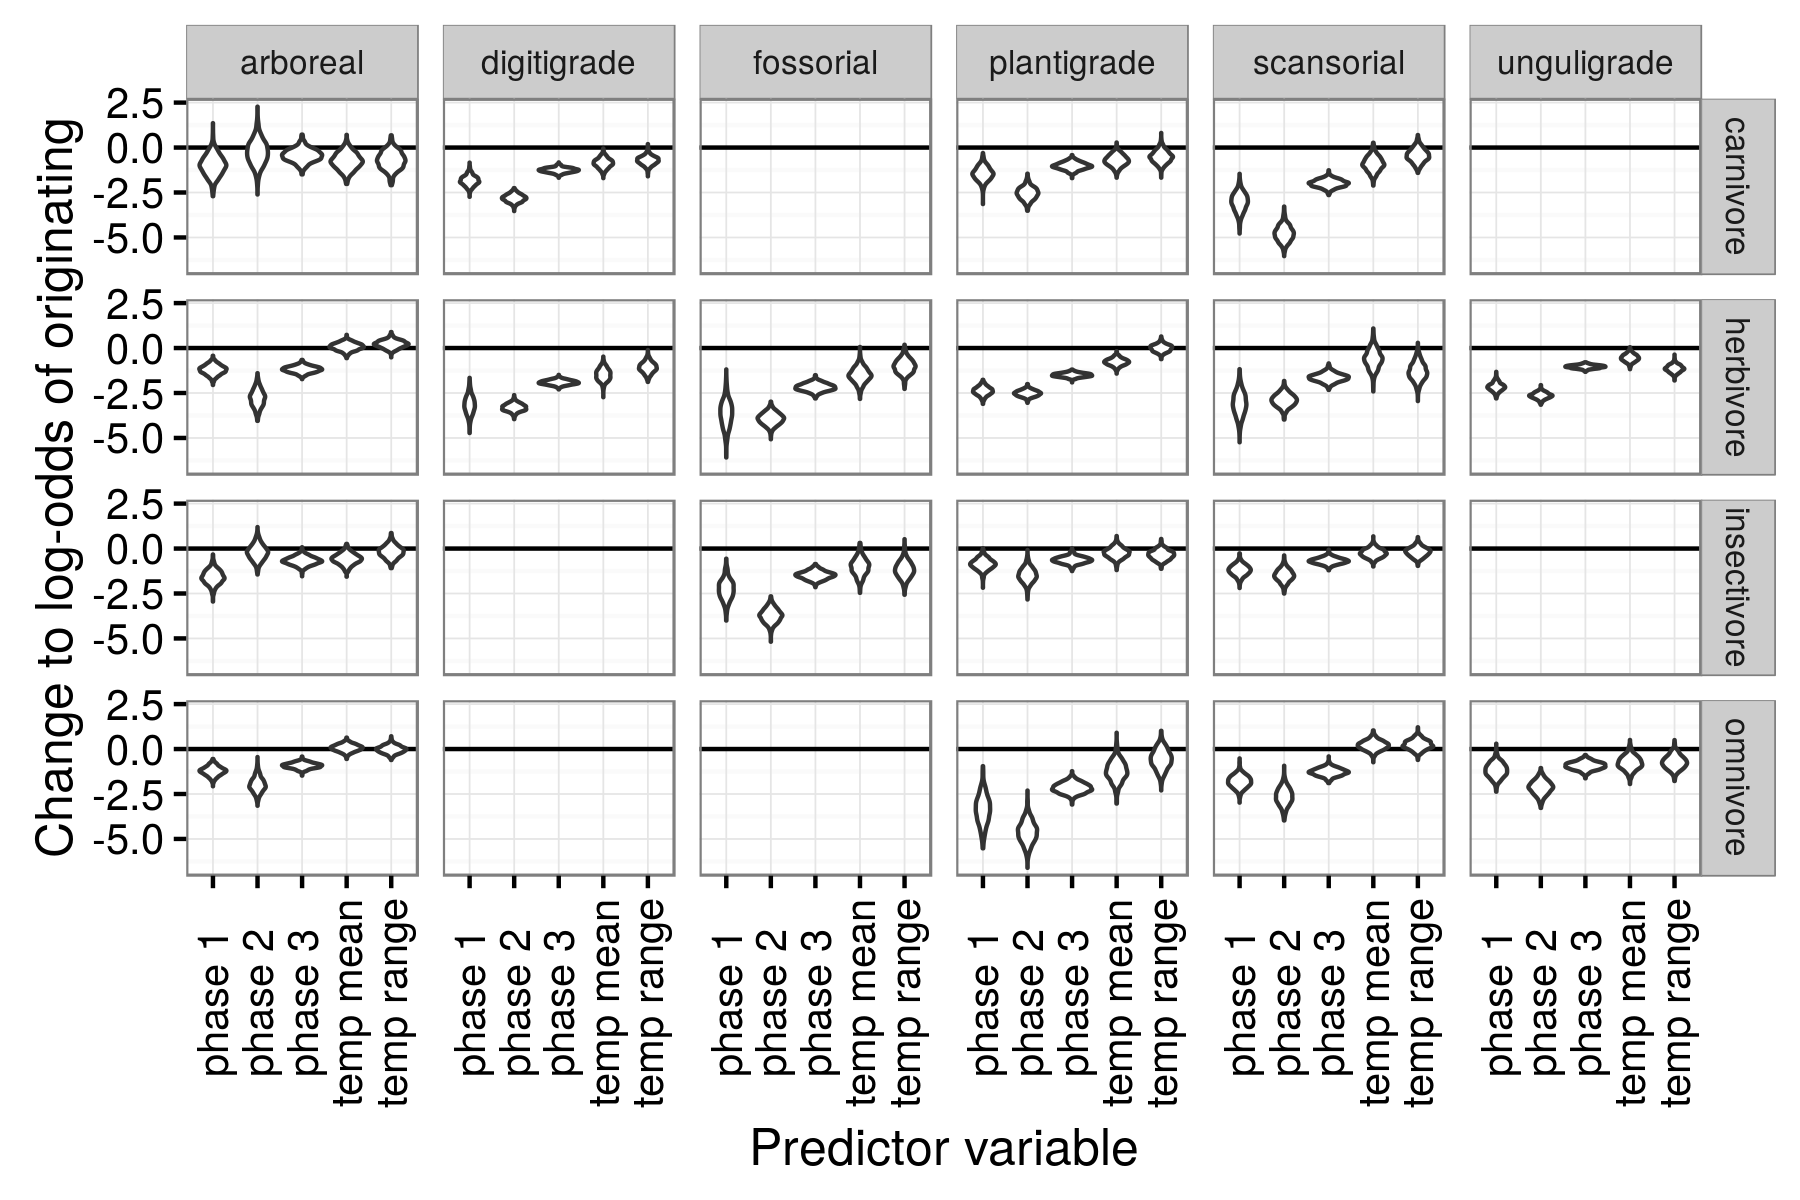
\includegraphics[height=0.8\textheight,width=\textwidth,keepaspectratio=true]{figure/group_on_origin_bd}
  \end{center}
\end{frame}

\begin{frame}
  \frametitle{Group-level effects (plant phase, climate) on survival}
  \begin{center}
    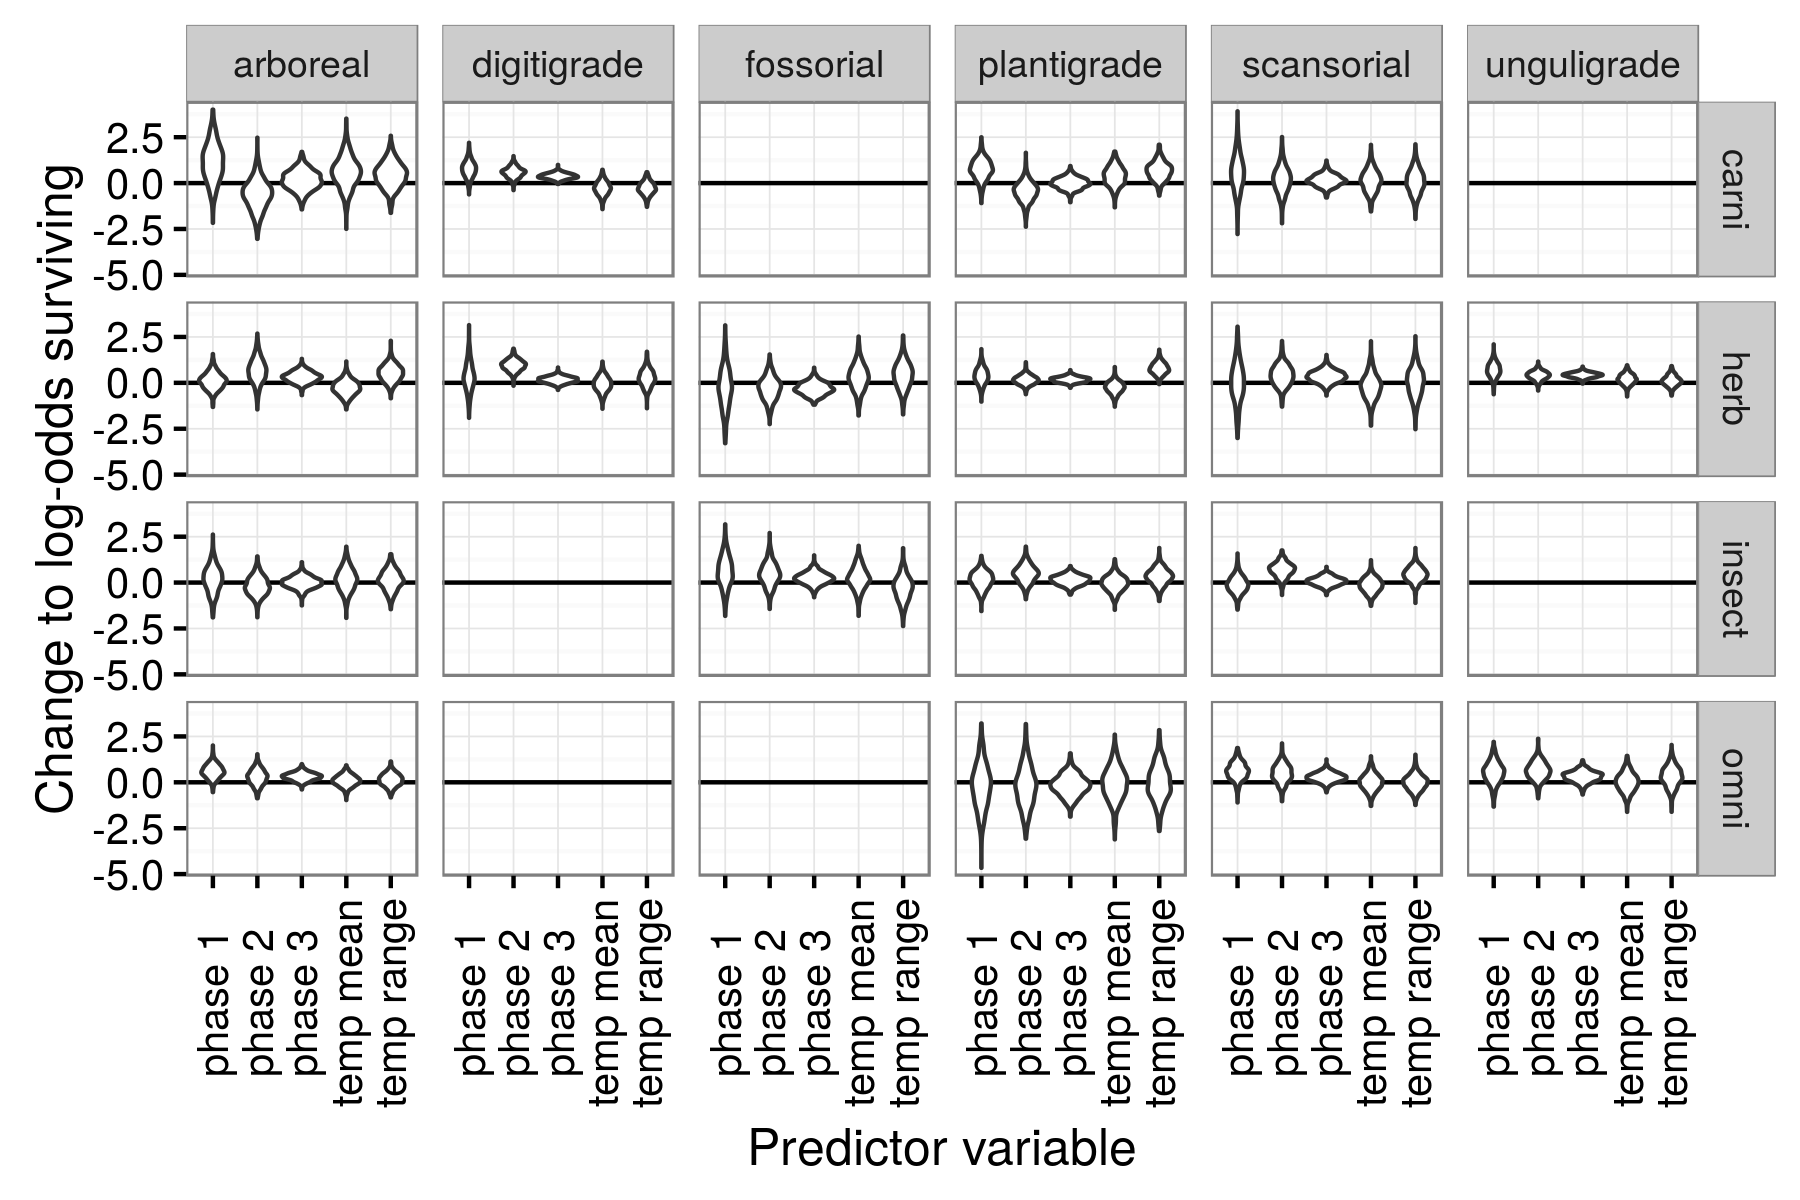
\includegraphics[height=0.8\textheight,width=\textwidth,keepaspectratio=true]{figure/group_on_survival_bd}
  \end{center}
\end{frame}

\begin{frame}
  \frametitle{Total species pool diversity and diversification}
  \begin{columns}
    \begin{column}{0.5\textwidth}
      \begin{center}
        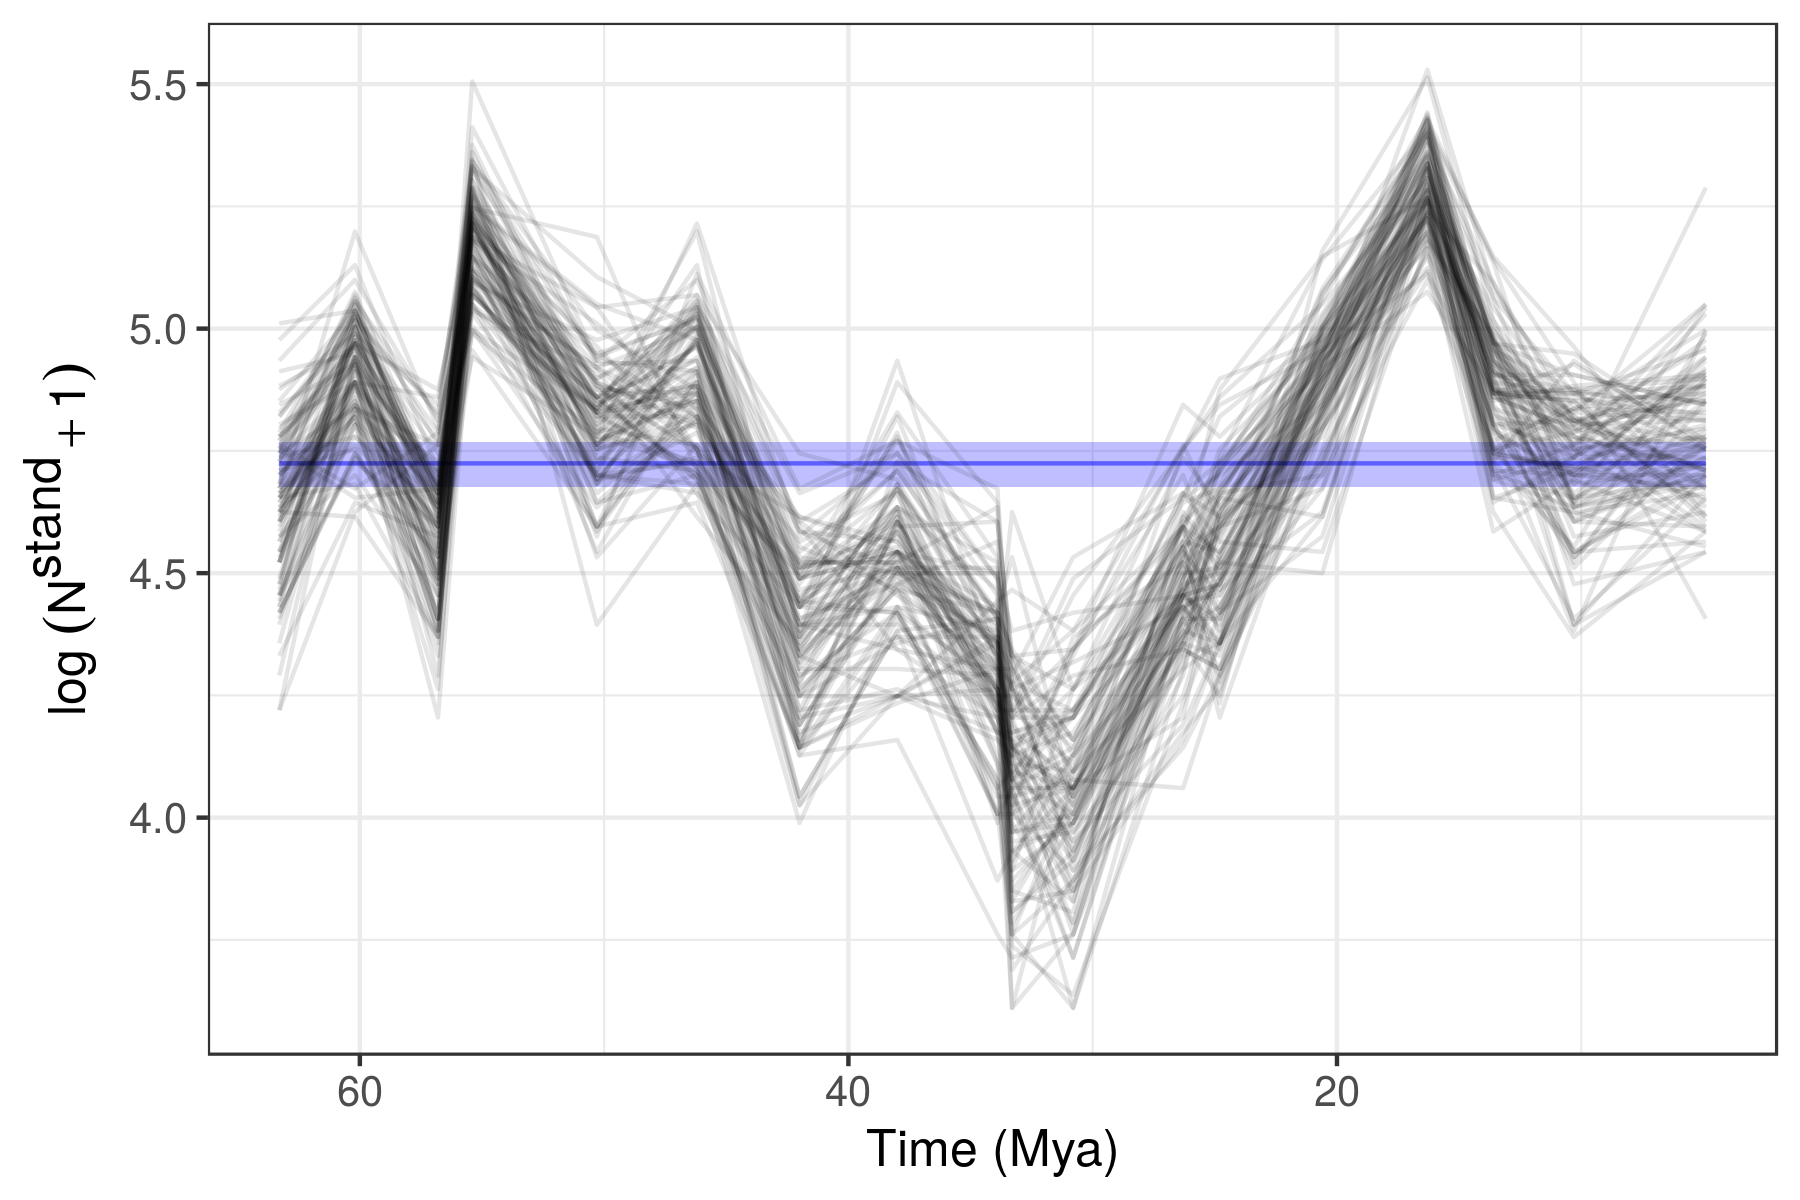
\includegraphics[height=0.4\textheight,width=\textwidth,keepaspectratio=true]{figure/log_diversity}

        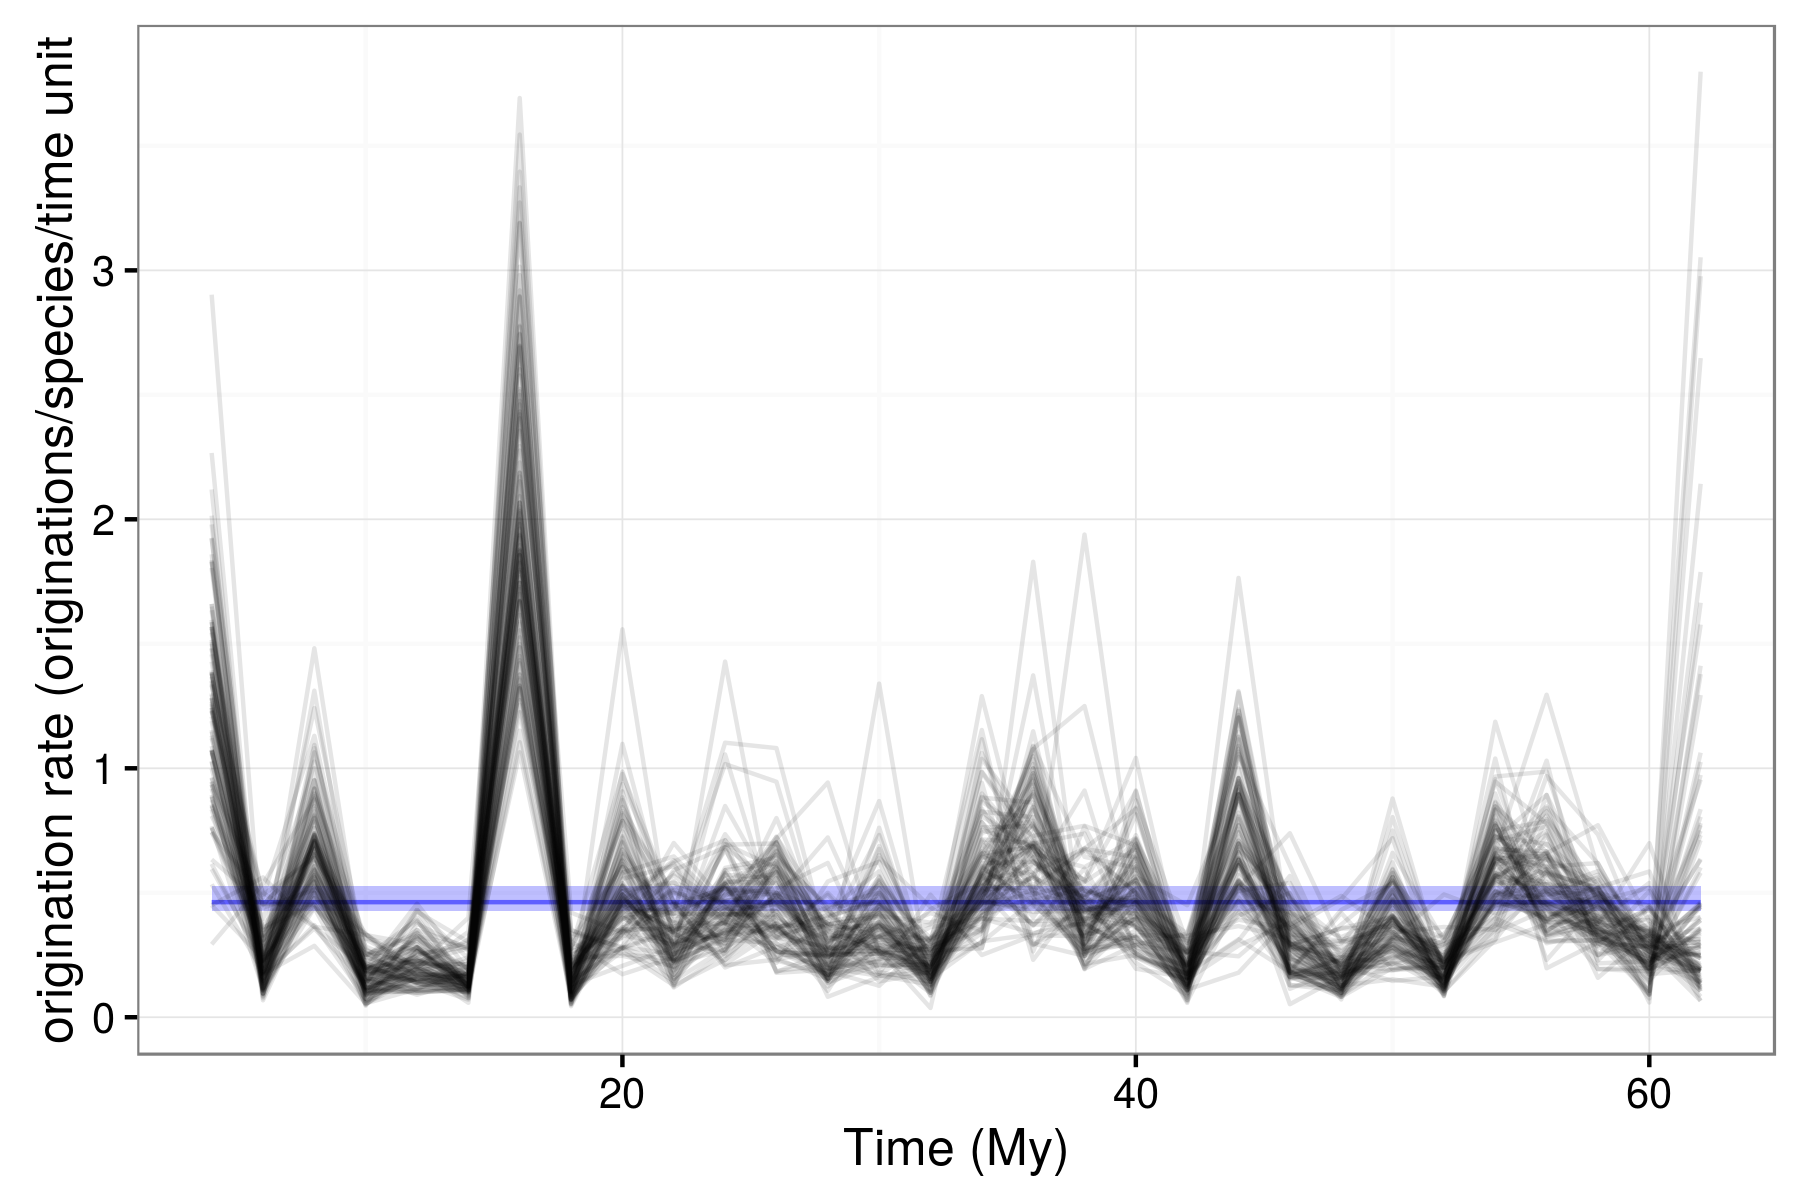
\includegraphics[height=0.4\textheight,width=\textwidth,keepaspectratio=true]{figure/orig_rate}
      \end{center}
    \end{column}
    \begin{column}{0.5\textwidth}
      \begin{center}
        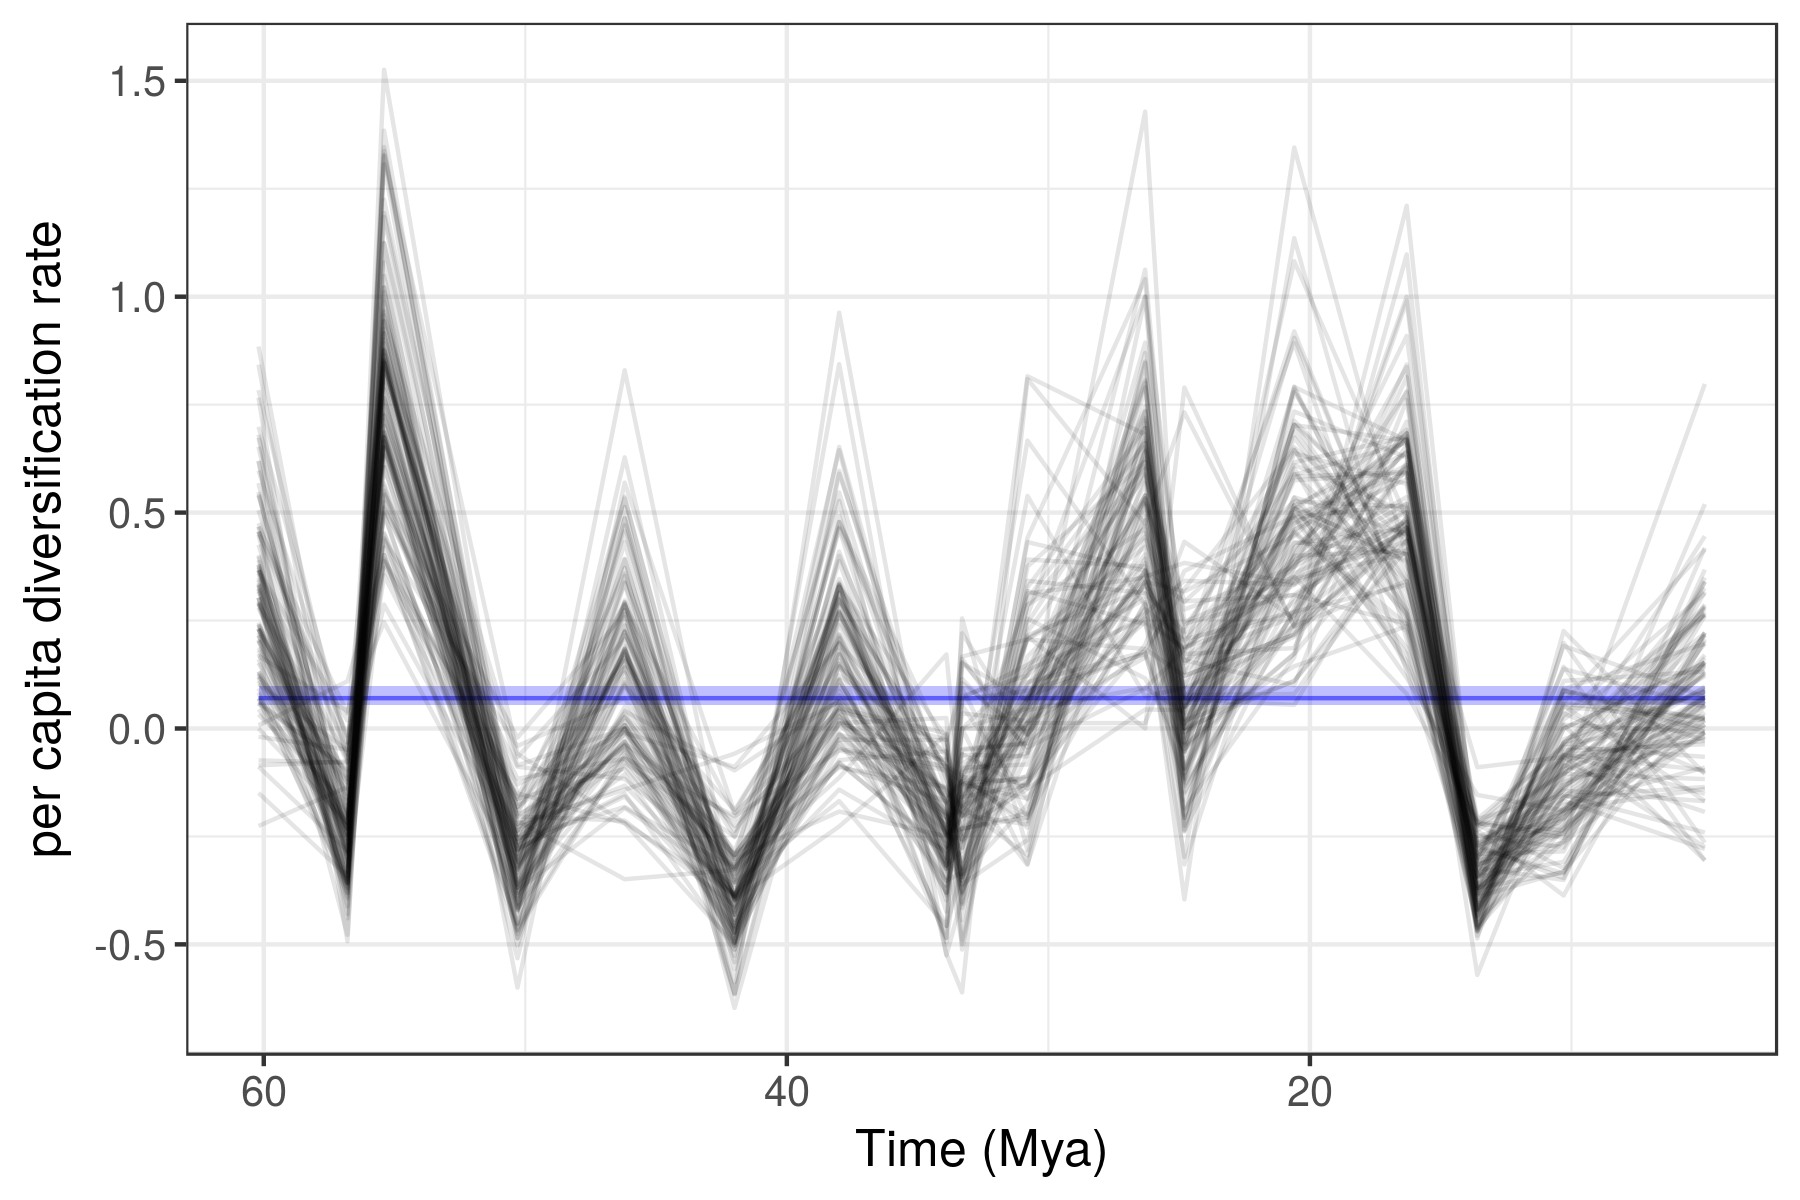
\includegraphics[height=0.4\textheight,width=\textwidth,keepaspectratio=true]{figure/div_rate}

        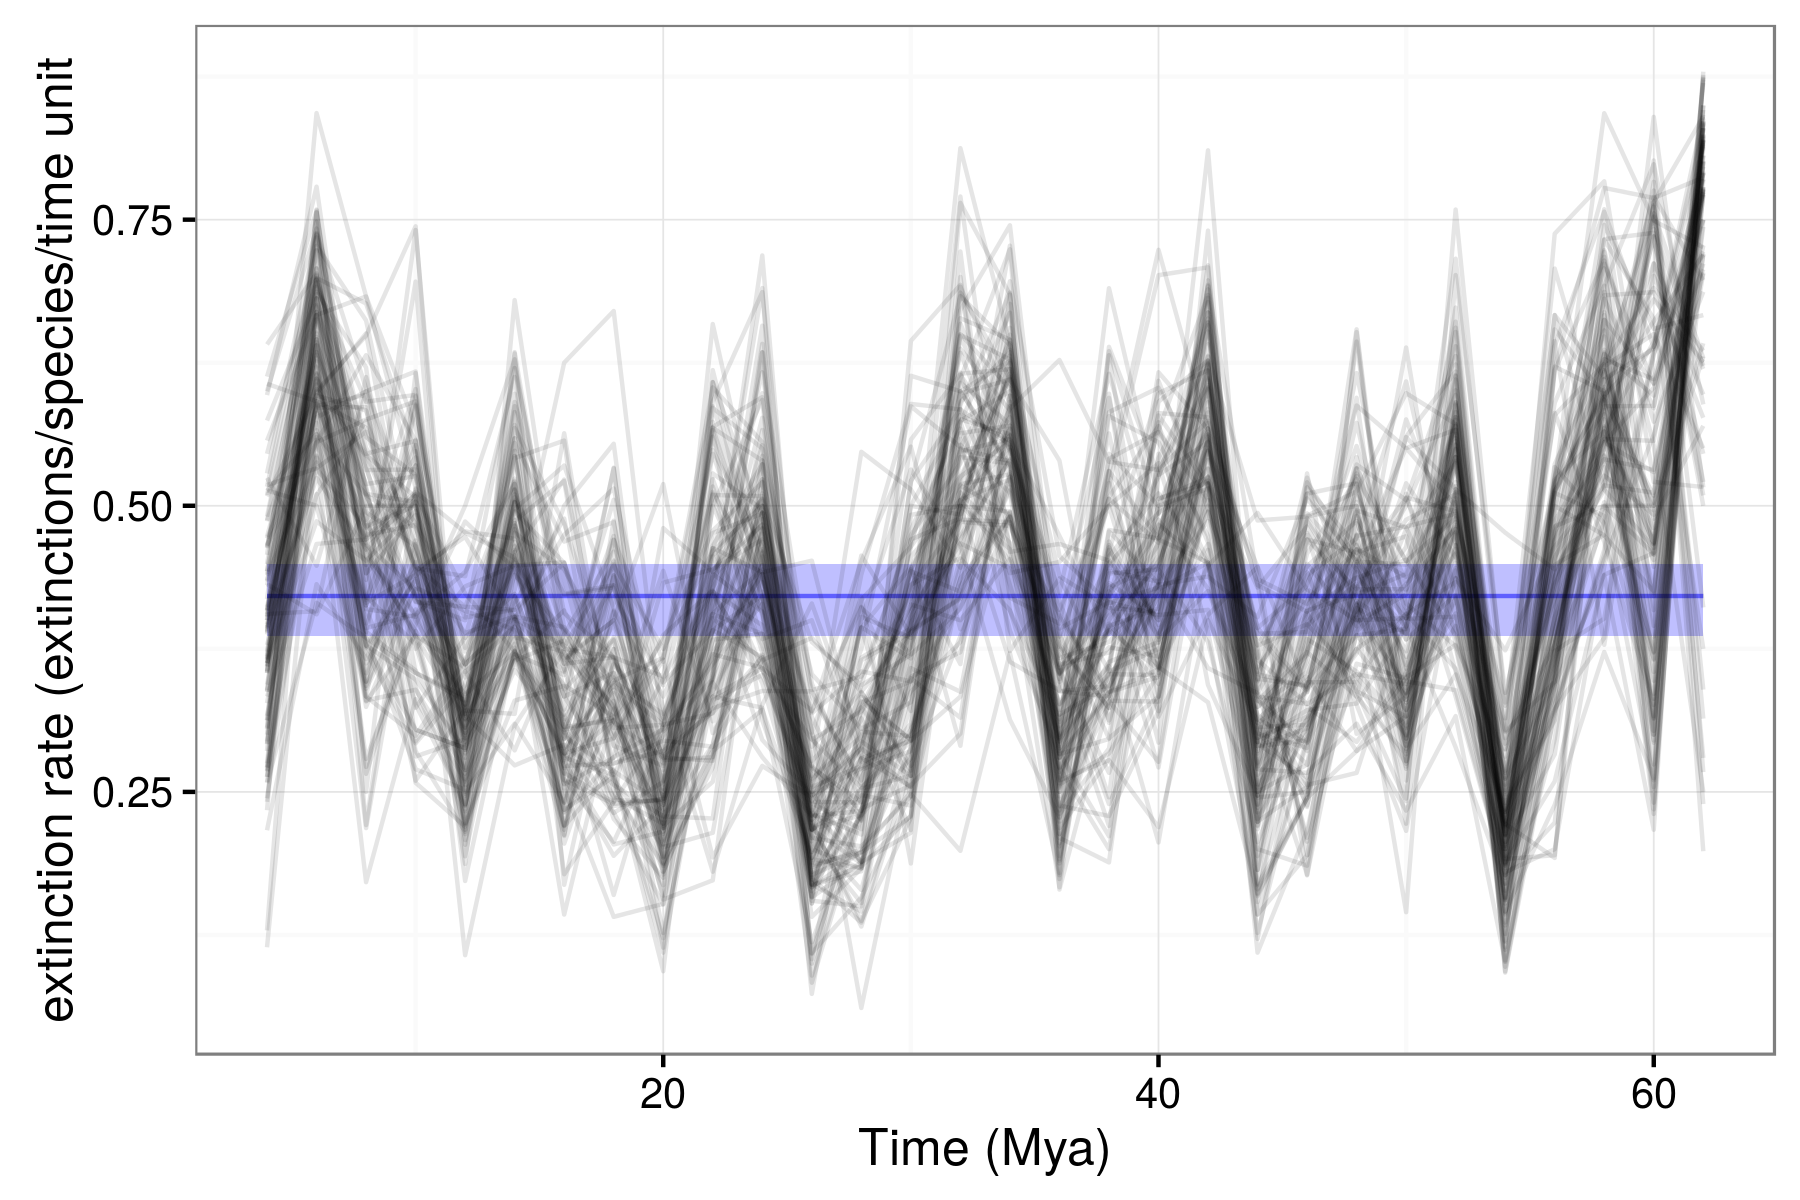
\includegraphics[height=0.4\textheight,width=\textwidth,keepaspectratio=true]{figure/death_rate}
      \end{center}
    \end{column}
  \end{columns}
\end{frame}

\begin{frame}
  \frametitle{Ecotype-specific diversity}
  \begin{center}
    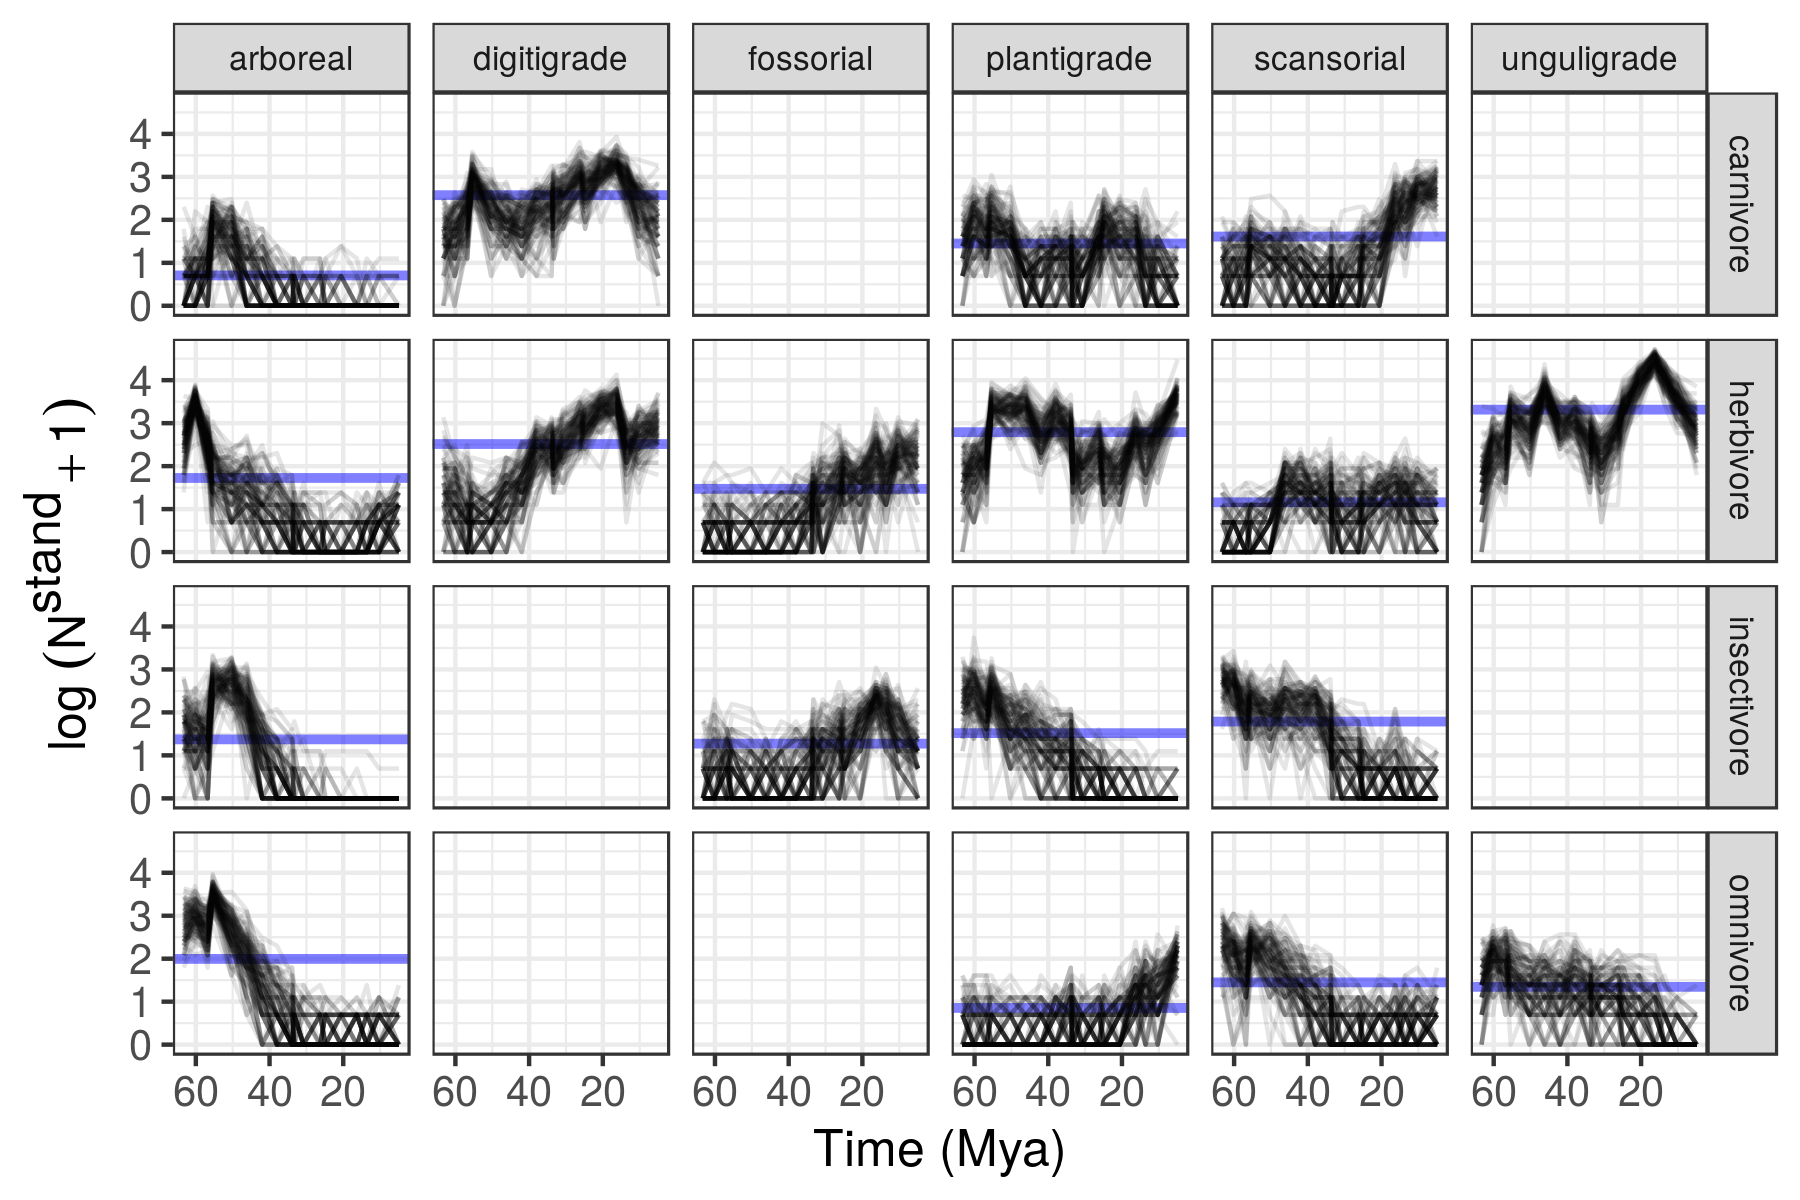
\includegraphics[height=0.8\textheight,width=\textwidth,keepaspectratio=true]{figure/ecotype_diversity}
  \end{center}
\end{frame}

%\begin{frame}
%  \frametitle{Ecotype-specific origination}
%  \begin{center}
%    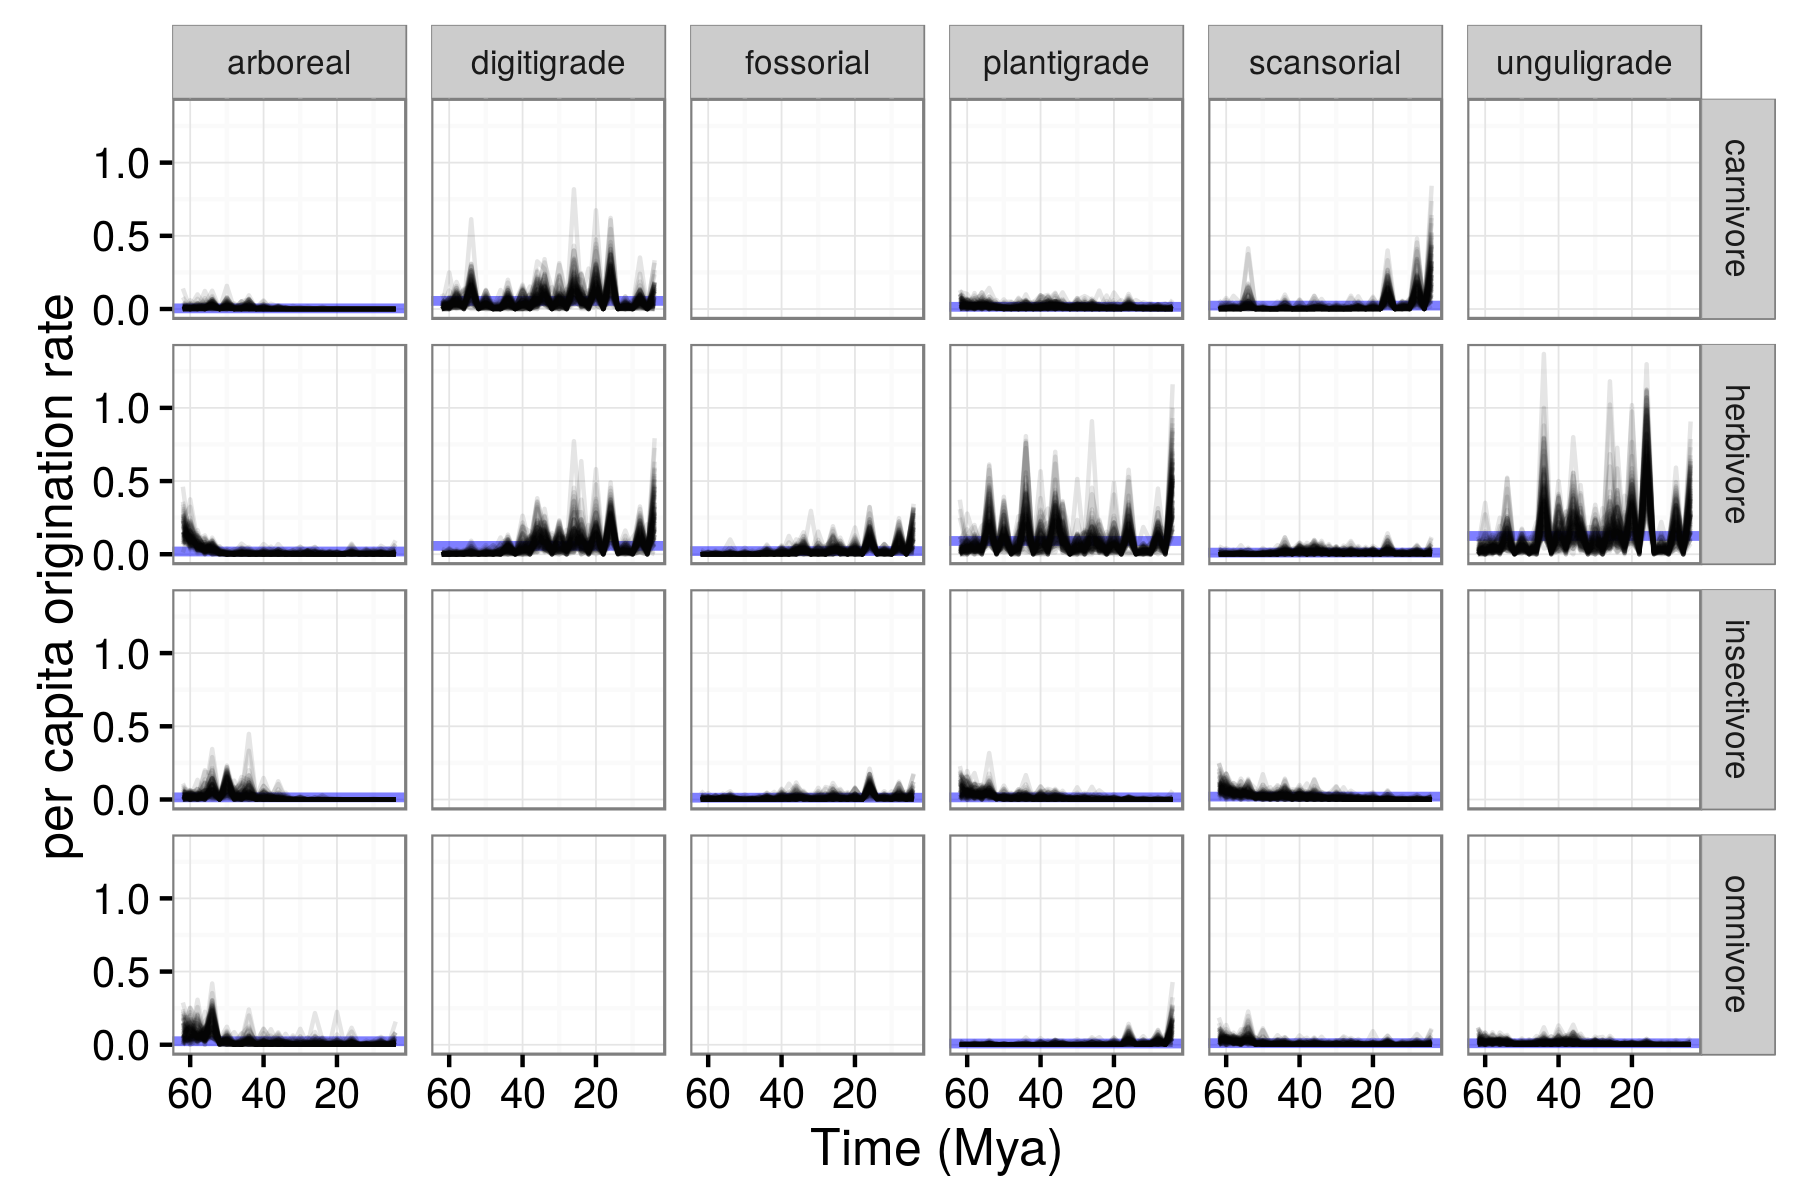
\includegraphics[height=0.8\textheight,width=\textwidth,keepaspectratio=true]{figure/birth_eco}
%  \end{center}
%\end{frame}
%
%\begin{frame}
%  \frametitle{Ecotype-specific extinction}
%  \begin{center}
%    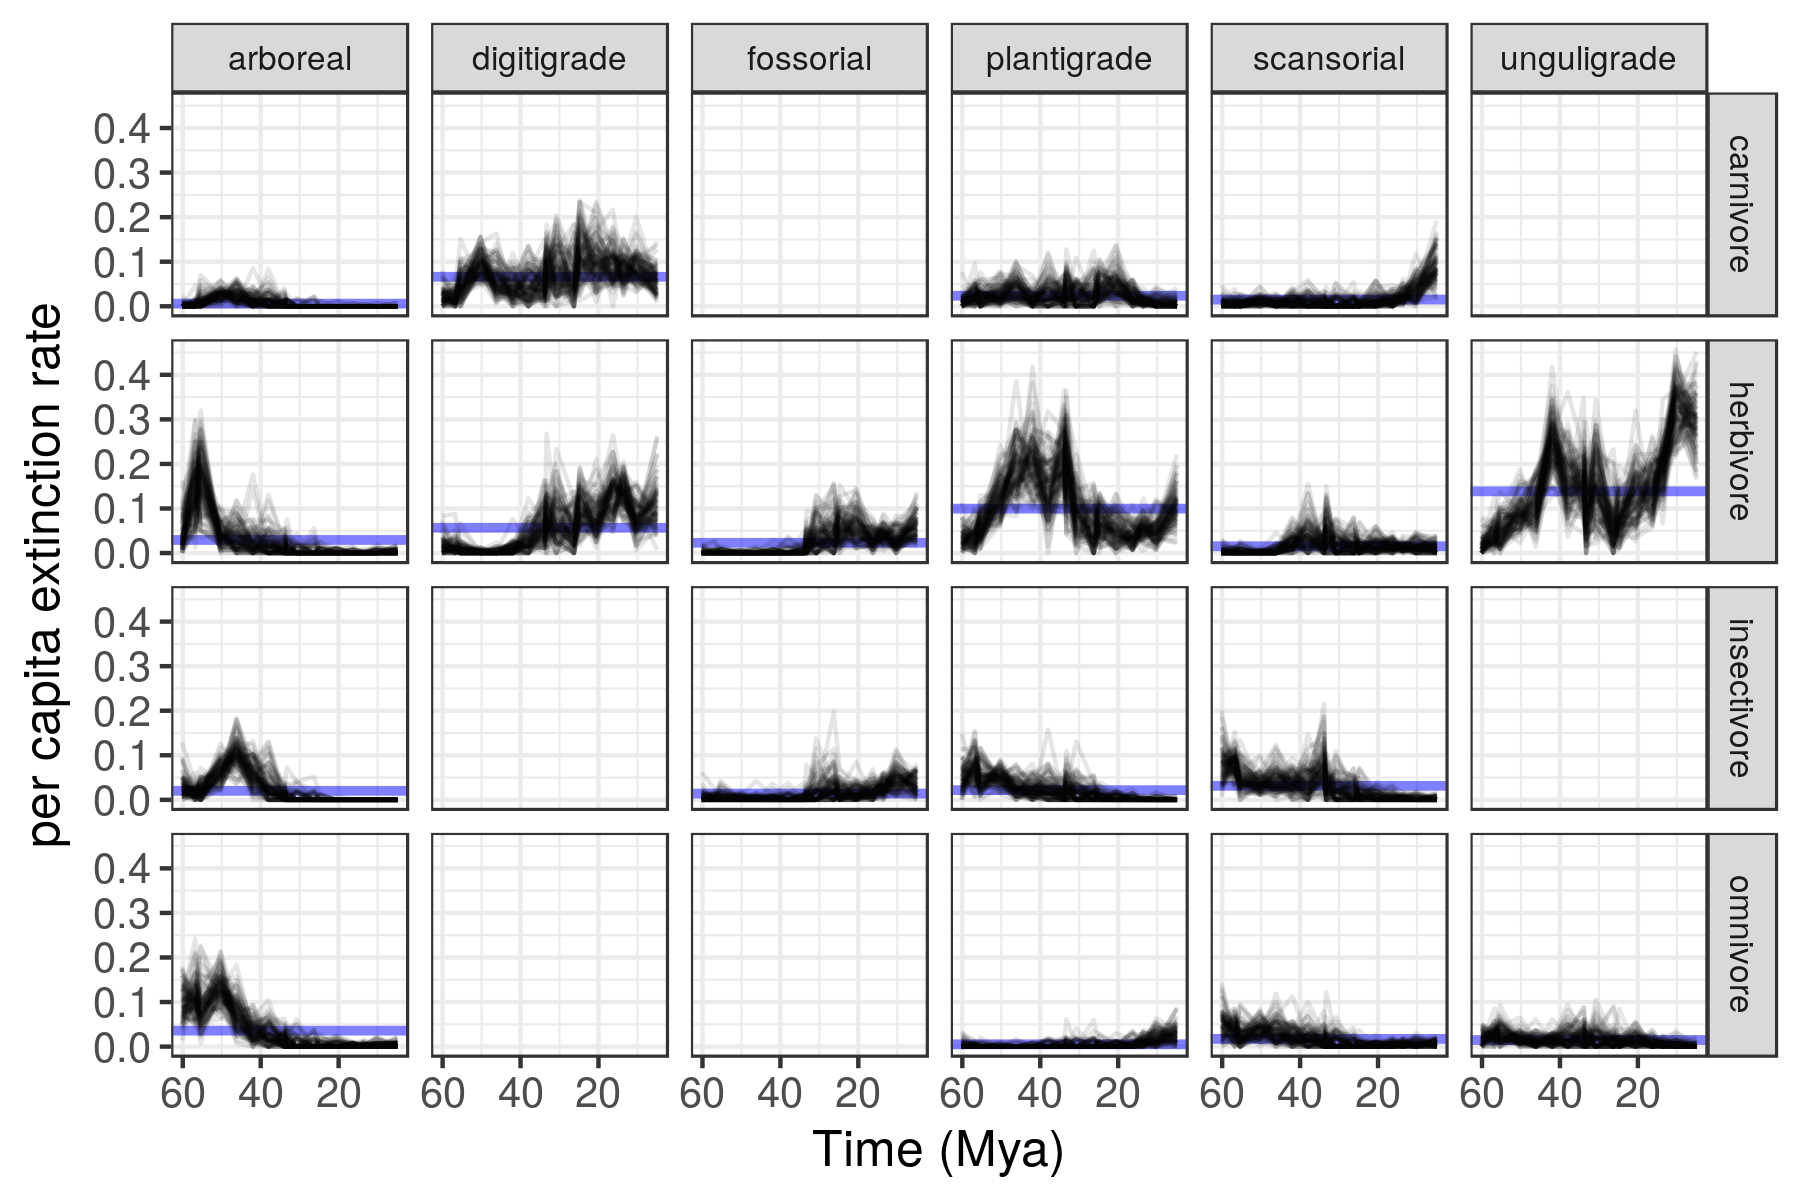
\includegraphics[height=0.8\textheight,width=\textwidth,keepaspectratio=true]{figure/death_eco}
%  \end{center}
%\end{frame}

\begin{frame}
  \frametitle{Relative ecotype diversity}
  \begin{center}
    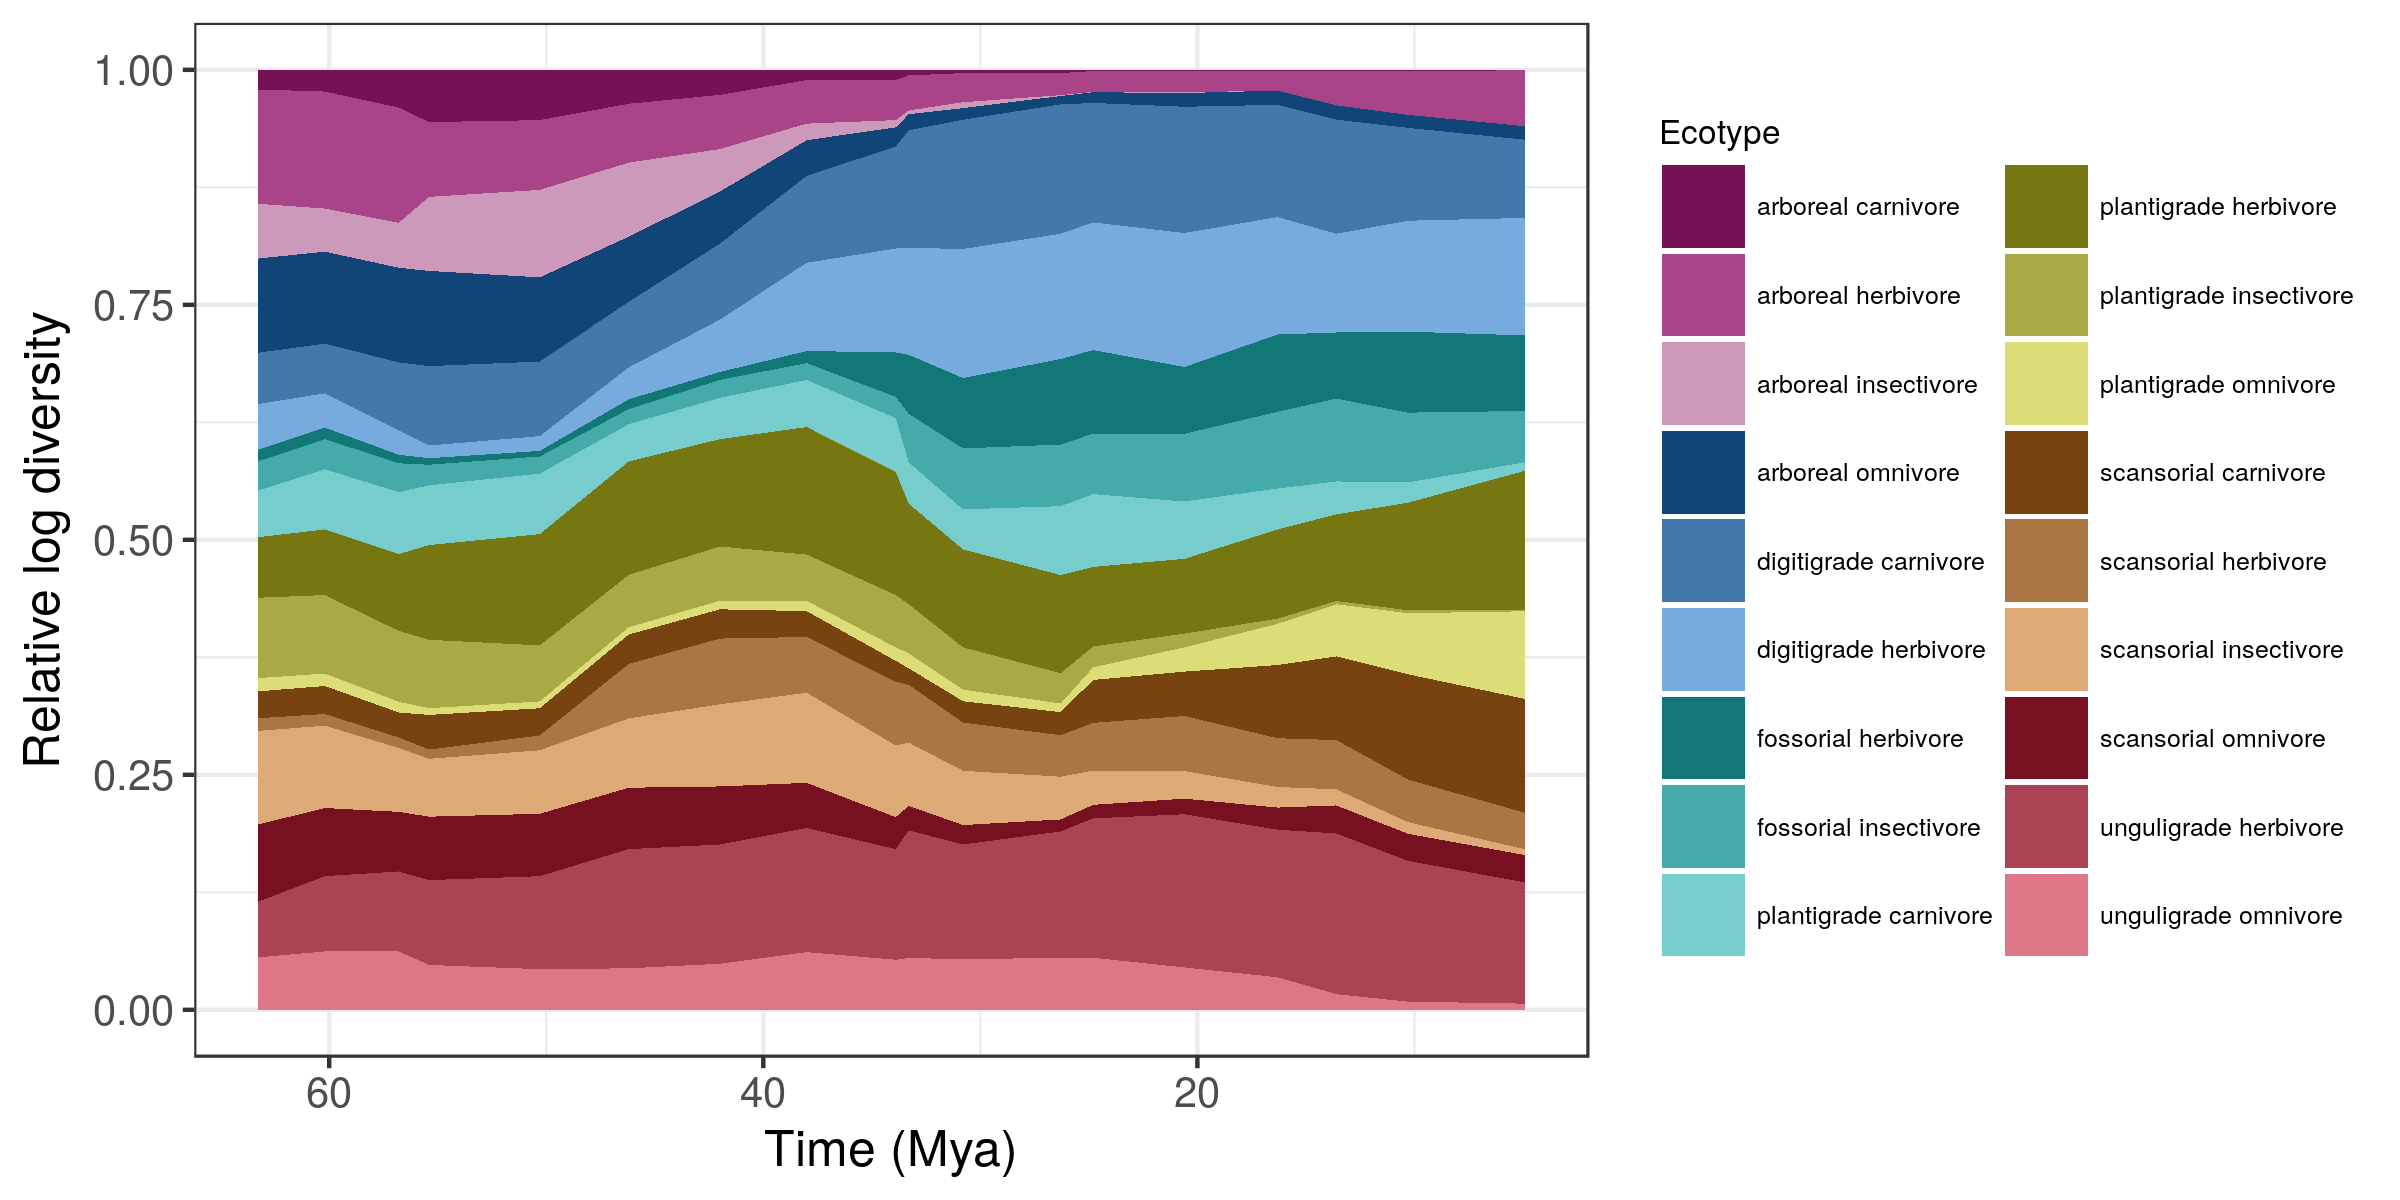
\includegraphics[height=0.8\textheight,width=\textwidth,keepaspectratio=true]{figure/relative_diversity}
  \end{center}
\end{frame}

\begin{frame}
  \begin{block}{Summary of results}
    \begin{itemize}
      \item changes to ecotype composition driven by origination, not extinction
        \begin{itemize}
          \item specific ecotypes source of most variation in overall origination
        \end{itemize}
      \item arboreal taxa decrease through Paleogene, all but absent by Neogene
      \item digitigrade and unguligrade herbivores only groups with sustained increase
      \item environmental covariates virtually always affect origination, not survival
    \end{itemize}
  \end{block}
\end{frame}




\begin{frame}
  \frametitle{Acknowledgements}
  \begin{columns}
    \begin{column}{0.5\textwidth}
      \begin{itemize}
        \item Advising
          \begin{itemize}
            \item Kenneth D. Angielczyk, Michael J. Foote, \\P. David Polly, \\Richard H. Ree, \\Graham Slater
          \end{itemize}
        \item Angielczyk Lab
          \begin{itemize}
            \item {\small{David Grossnickle, \\Dallas Krentzel, \\Jackie Lungmus}}
          \end{itemize}
        \item Foote lab
          \begin{itemize}
            \item {\small{Marites Villarosa Garcia, \\Nadia Pierrehumbert}}
          \end{itemize}
      \end{itemize}
    \end{column}
    \begin{column}{0.5\textwidth}
      \begin{itemize}
        \item {\footnotesize{David Bapst, Ben Frable, \\Graeme Lloyd, Matt Pennell}}
        \item {\footnotesize{UChicago CEB}}
      \end{itemize}

      \vspace*{0.05\textheight}
      \begin{center}
        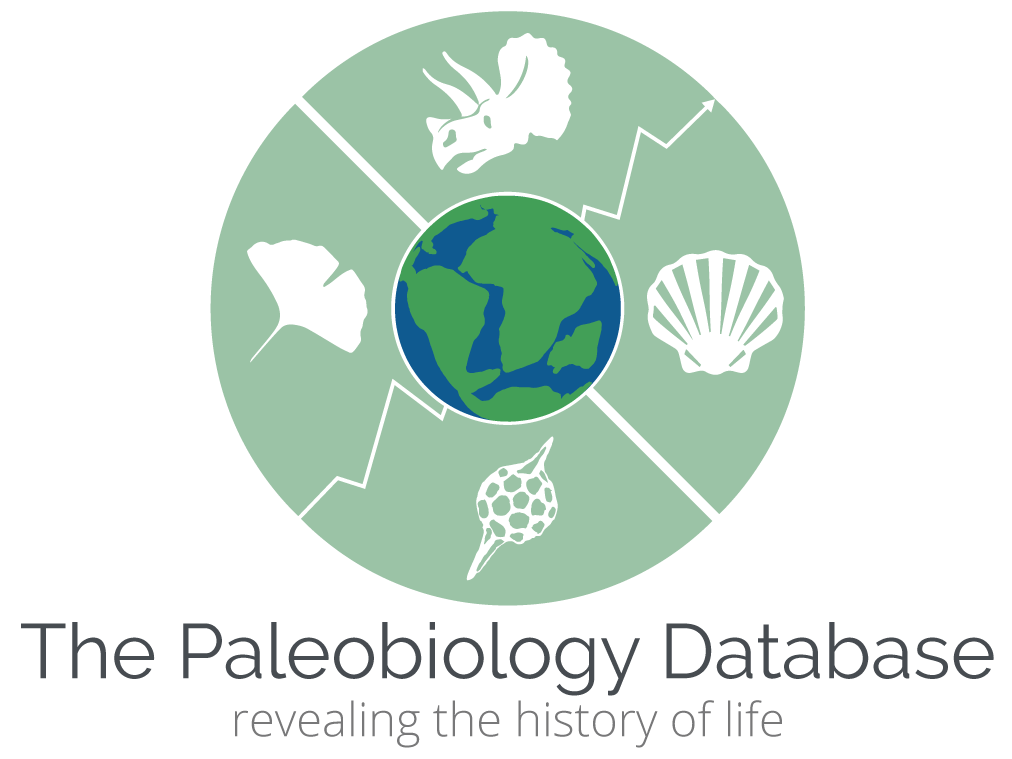
\includegraphics[height=0.4\textheight,width=\textwidth,keepaspectratio=true]{figure/paleodb}
      \end{center}
    \end{column}
  \end{columns}
\end{frame}

\end{document}

